\documentclass[a4paper,openany,11pt]{book}


%%includes and style stuf 
	\usepackage{nameref}
	\usepackage[dvipsnames]{xcolor}
	\usepackage{graphicx} 
	\graphicspath{{Figures/}}
	\usepackage[left=1in,right=1in,top=0.5in,bottom=0.8in]{geometry}
	\usepackage[breaklinks]{hyperref}
	\usepackage{microtype}
	\usepackage{tikz}
	\usepackage{natbib}
	\usepackage{multicol}
	\usepackage{amsmath}
	\usepackage{amssymb}
	\usepackage{JML}
	\usepackage{tikz}
	\usepackage{pgfplots}
	\usepackage{wrapfig}
	\newcommand\cec[1]{\tilde{\vec{#1}}}
	\usetikzlibrary{decorations.pathreplacing,calligraphy}
	\usepackage[framemethod=tikz]{mdframed}
	\mdfdefinestyle{mpdframe}{
		frametitlebackgroundcolor   =black!15,
		frametitlerule          =true,
			roundcorner     =10pt,
			middlelinewidth     =1pt,
			innermargin     =.20cm,
			outermargin     =0.2cm,
			innerleftmargin     =0.2cm,
			innerrightmargin        =0.2cm,
			innertopmargin      =\topskip,
			innerbottommargin   =\topskip,
				}
	%   Studies
	\mdfdefinestyle{a}{%
			style=mpdframe,
			frametitle={Aside},
		}

		% \newcommand\inner[2]
		% {
		% 	\langle \vec{#1}, \vec{#2} \rangle
		% }
	\newmdenv[style=a]{aside}
	\setlength\parindent{0pt}
	\setlength\parskip{8pt}

\title{First Principles of Machine Learning \\ Notes}
\author{Jack Fraser-Govil}
\date{October 2024}
\renewcommand\vec[1]{\boldsymbol{\mathbf{#1}}}
\def\t{^\intercal}
\begin{document}
	\maketitle

	\setcounter{tocdepth}{1}
	{\tableofcontents{}}	

	\part{Background Mathematics}


		\chapter{Introduction}

			{\large This section is designed to provide a brief overview of the background mathematics which will be touched upon during the workshop.

			It is \textbf{not} intended to be a comprehensive overview of the topics, and I will freely gloss over things that are uninteresting or irrelevant for the purpose at hand. This document is meant to be a quick reference guide, or a refresher for people who once knew these things, but have long since forgotten them. 

			If you read nothing else, it will be vitally important for you to have a grasp of the \textbf{chain rule}, since this is the cornerstone of backpropagation. Similarly, understanding Matrix multiplication (even if you can't actually do it by hand) and the dot product will be of vital importance for our work.}

			\section{Some Basic Notation}

				I will be using (mostly) formal mathematical notation throughout, but will endeavour to ensure that whenever notation is first introduced,  it is explained. I will also ensure that the surrounding text explains what is going on such that you should be able to gather from context clues what an expression means. 

				That being said, some basic notation is helpful to get out of the way:

				\begin{itemize}
					\item Scalar quantities (i.e. simple numbers and placeholders), will be written in lower case italics. $x$, $y$, $z$ and so on. 
					\begin{itemize}
						\item An exception to this is \textit{scaling parameters} (i.e. numbers which control how large a function is) will be written in curly fonts, $\mathcal{N}, \mathcal{A}$ if we don't actually care about their value.
						\item Functions will also be written in lower case italics; $y = f(x)$\footnote{Technically I should reserve this for 'scalar functions' (where the output is a scalar); and let vector functions be written as $\vec{f}(x)$, for example. For simplicity, I won't do this: all functions will be written the same.}.
					\end{itemize}
					\item Vector quantities will be written in boldface. $\vec{x}$, $\vec{y}$, $\vec{a}$.
					\begin{itemize}
						\item Since \textit{elements} of a vector are (usually) scalars, they will be written in italics. $a_i$ = $[\vec{a}]_i$ is the $i^\text{th}$ element of the vector $\vec{a}$.
					\end{itemize}
					\item Matrices (and Linear Operators) will be written in capital italics; $M, N, P$ and so on.
					\item Derivatives will usually be written in Newton's Notation ($\div{y}{x}$), but I will sometimes use Leibniz's notation ($f^\prime(x)$) if the text is getting a bit cramped! This is purely a stylistic choice. Don't read into it.
				\end{itemize}
		

		\chapter{Calculus}

			Calculus is the mathematical study of \textit{change}. It is needed in order to study how a function varies as its inputs are altered. For the purposes of machine learning, therefore, it is of vital importance in the process of optimization, since we are (hopefully) trying to alter the parameters of a model until the loss function reaches a maximum: this is a process only possible via calculus. 

			\section{Functions}

				The notation and theory which underlies even the simplest of functions is vast and complex (Real Analysis), and is a field where trivial-sounding statements are often impossible to prove. 
				
				Luckily, we don't need any of that. 

				For our purposes, it is sufficient to note that a function is any form of \textbf{mapping} between two sets of objects. It is common for these sets to be two different kinds of numbers: for instance the function $f(x) = x^2$ maps all (real) numbers to the set of all positive numbers. However, there is no general restriction that a function `only' has to be a relationship between numbers. 

				A function is a black box, into which you put an input, and you receive an output. We denote this as:

				\begin{equation}
					y_\text{output} = f(x_\text{input})
				\end{equation}
				Here $x$ and $y$ can be anything; $x$ might be a particular scent, and $y$ could be the U2 album that smell most reminds my Dad of. In general, however, we will be most interested in cases where these are numerical quantities: either vectors or scalars. 



				\subsection{Continuity}

					A function is said to be \textbf{continuous at a point} if it obeys the following relationship:

					\begin{equation}
						\lim_{x \to c}\left(f(x)\right)  = f(c)
					\end{equation}
					That is, the limit of the function is the same as the value of the function. This definition also implicitly requires that the limit be the same \textit{no matter which direction you approach from}.

					\begin{center}
						\begin{tikzpicture}
						
						\begin{axis}[xmin = -2, xmax = 2, ymin = -3, ymax = 1.2, ylabel={$y$ }, xlabel ={$x$},x post scale = 1]
										\addplot[domain = -2:0, samples = 200,blue]{x};
										\addplot[domain = 0:2, samples = 200,blue]{1-x};
									\end{axis}
						
						\end{tikzpicture}
						\end{center}
					The function above is therefore non-continuous at $x = 0$ because the limit has different values depending on if you approach from the left or the right. 

					`Continuity' is therefore a fancy way of saying `if you draw the function as a graph, you don't have to take your pen off the page' -- however this definition generalises to arbitrary quantities where you can meaningfully define limits (such as 24-dimensional spaces where your pencil would have to curl in on itself).

				\subsection{Nested or Chained Functions}

					It will be exceptionally common (and very important for us!) to consider the cases where functions are nested. If $f$ and $g$ are both functions from some `object space'\footnote{A field} $F$ to the same space (i.e. the output is the same type of object as the input), then it is possible to have:
					\begin{equation}
						y = f(g(x))~~~~ \leftrightarrow~~~~ y = f\circ g\circ x
					\end{equation}
					(This $\circ$ notation is a functional notation some mathematicians like. It cuts down on parentheses.) This should be read as ``do $g$ to $x$ first, and then do $f$ to the output of that''.

					Many more complex mathematical expressions can be written as nestings of more simple functions; for instance the Gaussian function \textit{can} be written as:
					\begin{equation}
						y = \mathcal{N} \exp\left(- \frac{1}{2} \left( \frac{x - \mu}{\sigma}\right)^2\right)
					\end{equation}
					Or it can be written as:
					\begin{align}
						y(x) & = \mathcal{N} f(g(h(x)))
						\\
						f(g) & = \exp(g)
						\\
						g(h) & = -\frac{1}{2} h^2
						\\
						h(x) & = \frac{x - \mu}{\sigma}
					\end{align}

			\section{Derivatives}

				We will now assume that we are dealing solely with real functions; those where the inputs and outputs are both real numbers. When you have such a function, it is natural to ask ``how does the output change when I change the input?''.

				This is the \textbf{gradient} of the function: for a function $y = f(x)$, it is the amount that $y$ changes, when $x$ changes by a small amount. 

				It is clear that the answer to this question varies, depending where you are looking. In the plot below, the gradient at $x = 0$ (the first red dot) is clearly very flat; the value of the function at $x = 0.1$ is 0.01; very close to zero, and so the function has not changed that much. At $x = 1.5$ (and $y = 2.25$), however, the gradient is much steeper: increasing $x$ by 0.1 increases $y$ by 0.31 -- 31 times larger than the increase we saw at $x = 0$!

				\begin{center}
					\begin{tikzpicture}
					
					\begin{axis}[xmin = -2, xmax = 2, ymin = -1, ymax = 5, ylabel={$y$ }, xlabel ={$x$},x post scale = 1]
									\addplot[domain = -2:2, samples = 200,blue]{x^2};
									%  \addplot[domain = 0.5:1.5, samples = 2, red, ultra thick]{2*x - 1};
									\addplot[mark=*, red] coordinates {(0,0)};
									\addplot[mark=*, red] coordinates {(1.5,2.25)};

									% \addplot[domain = 0.5:1.5, samples = 2, green,ultra thick]{2*x - 0.75};
									%  \addplot[mark=*, green] coordinates {(-1,1)};
									%  \addplot[domain = -1:1, samples=2, orange, ultra thick]{0};
									%  \addplot[mark=*, orange] coordinates {(0,0)};
								\end{axis}
					
					\end{tikzpicture}
					\end{center}

				The gradient of $f(x)$ is therefore a second function; when evaluated at $x$ it tells you how steep the original function is at that point. This gradient function is the \textit{derivative} of the function, and is denoted:
				\begin{equation}
					\text{gradient of $f$ at }x = \div{f}{x} = f^\prime(x)
				\end{equation}

				\subsubsection{Isn't that a fraction?}
				Despite being written using familiar notation, mathematicians will generally start shouting at you if you treat $\div{f}{x}$ like a fraction. They'll start howling about things like `infinitesimals' and `surreal numbers'.
				
				The dirty secret that mathematicians don't want you to know is that it is \textit{often perfectly fine} to do so with single-valued functions, and things behave as intuitively as you might expect:
				\begin{align}
					\div{x}{x} & = 1
					\\
					\frac{1}{\left(\div{y}{x} \right)} & = \div{x}{y}
					\\
					\div{f}{x}\d x & = \d f
				\end{align}
				However, when it comes to \textit{multivariable calculus}, and things start looking like $\pdiv{f}{x}$, then you should never treat them as fractions.

				\subsection{Formally Defining the Derivative}

					Even though it's not strictly necessary, it can often be helpful to recall the formal definition of the derivative. 

					Consider a function $f(x)$ which you are able to calculate, but you would like to know the \textbf{gradient} of. In the absence of any other ideas, tt is reasonable to try and estimate the gradient using a \textbf{chord}. 
					
					To do this, we choose a point $\Delta x$ away from $x$, and then draw a line between the two points.  An example of this is shown in Fig. \ref{F:Chord1}.
					\begin{figure}
						\begin{center}
						\begin{tikzpicture}
						
						\begin{axis}[xmin = -2, xmax = 2, ymin = -1, ymax = 5, ylabel={$y$ }, xlabel ={$x$},x post scale = 1]
										\addplot[domain = -2:2, samples = 200,blue]{x^2};
										%  \addplot[domain = 0.5:1.5, samples = 2, red, ultra thick]{2*x - 1};
										\addplot[mark=*, red] coordinates {(0.5,0.25)};
										\addplot[mark=*, red] coordinates {(1.5,2.25)};

										\addplot[domain = 0.5:1.5, samples = 2, green,ultra thick]{2*x - 0.75};
										%  \addplot[mark=*, green] coordinates {(-1,1)};
										%  \addplot[domain = -1:1, samples=2, orange, ultra thick]{0};
										%  \addplot[mark=*, orange] coordinates {(0,0)};
									\end{axis}
						
						\end{tikzpicture}
						\end{center}
						\caption{\small A Chord-approximation using $x_1 = 0.5$ and $x_2 = 1.5$}\label{F:Chord1}
					\end{figure}
						The gradient of this choord can easily be computed as:
						\begin{equation}
							g = \frac{\Delta y}{\Delta x} = \frac{f(1.5) - f(0.5)}{(1.5) - (0.5)}
						\end{equation}
						Since (in this case) $f(x) = x^2$, this simplifies down to:
						\begin{equation}
							g = \frac{2.25 - 0.25}{1} =2
						\end{equation}
						Therefore the gradient \textit{of the chord} is equal to 2; but we can see that this isn't quite the gradient of the function -- the chord is much steeper! The chord is merely an approximation to the true gradient.
						

						If we reduce $\Delta x$, then maybe we get a better approximation (see Fig \ref{F:Chord2}):
						\begin{align}
							\begin{split}
							g & = \frac{\Delta y}{\Delta x} 
							\\
							& = \frac{f(0.75) - f(0.5)}{(0.75) - (0.5)}
							\\
							& = \frac{0.5625 - 0.25}{0.25}
							\\
							& = 1.25
							\end{split}
						\end{align}

						\begin{figure}
							\begin{center}
							\begin{tikzpicture}
							
								\begin{axis}[xmin = -2, xmax = 2, ymin = -1, ymax = 5, ylabel={$y$ }, xlabel ={$x$},x post scale = 1]
									\addplot[domain = -2:2, samples = 200,blue]{x^2};
									%  \addplot[domain = 0.5:1.5, samples = 2, red, ultra thick]{2*x - 1};
									\addplot[mark=*, red] coordinates {(0.5,0.25)};
									\addplot[mark=*, red] coordinates {(0.75,0.5625)};

									\addplot[domain = 0.25:1, samples = 2, green,ultra thick]{1.25*x - 0.375};
									%  \addplot[mark=*, green] coordinates {(-1,1)};
									%  \addplot[domain = -1:1, samples=2, orange, ultra thick]{0};
									%  \addplot[mark=*, orange] coordinates {(0,0)};
								\end{axis}
							
							\end{tikzpicture}
							\end{center}
							\caption{\small A Chord-approximation using $x_1 = 0.5$ and $x_2 = 0.75$}\label{F:Chord2}
						\end{figure}
						
						This is clearly much closer! We could repeat this exercise using the formula:
						\begin{equation}
							g \approx \frac{f(x + \Delta x) - f(x)}{\Delta x}
						\end{equation}
						If we repeat this with successively smaller $\Delta x$, we would (hopefully) eventually converge on the correct final answer. 

						\textbf{This is what differentiation is.} It is the above process, taken to the infinite limit where $\Delta x$ becomes infinitesimally small:
						\begin{equation}
							\frac{\d y}{\d x} = \lim_{\delta \to 0} \left( \frac{ f(x + \delta) - f(x)}{\delta} \right)
						\end{equation}

						Of course, the problem with this is that dividing by zero is undefined, so you can't just put $\delta = 0$ in here! The process works because, as you divide by zero, the number on the top \textit{also} becomes zero (because $f(x+\delta)$ and $f(x)$ become very similar) - so you are dividing an infinitely small value by another infinitely small value; in the hope that it cancels out, and you are left with something sane. 

						The joy of the above definition is that you don't \textbf{actually} need to care about it -- it is the formal definition of a derivative, and can be helpful to remember what it means (especially when optimising). When dealing with an actual function, however, the derivatives are (usually) expressible in terms of other functions. 

						I won't prove these results now, but it can be shown that:
						\begin{align}
							\frac{\d}{\d x} & x^n  = n x^{n-1}
							\\
							\frac{\d}{\d x} & \cos(x)  = - \sin(x)
							\\
							\frac{\d}{\d x} & \log(x)  = \frac{1}{x}
							\\
							\div{}{x} & \exp(x) = \exp(x)
						\end{align}
						A discussion of how these values arise can be found in chapter \ref{Int:Polynomial}.

				\section{Properties of the Derivative}

					This can all seem quite complex and overwhelming, but the derivative is in fact a lovely object, and has a number of desirable properties.

					\subsubsection{It is a Linear Operator}

						This means that if you know the derivative of $f$ and the derivative of $g$, then:
						\begin{equation}
							\frac{\d}{\d x} \left(f(x) + \alpha g(x) \right) = \frac{\d f}{\d x} + \alpha \frac{\d g}{\d x}
						\end{equation}
						You can split apart sums, and pull constant functions out of the derivative, leaving you to focus on the nasty bits. 

					\subsubsection{It Vanishes at Maxima and Minima}

						Maxima or a Minima are, by definition, the local extrema of a function -- they are (locally) the highest or lowest values the function achieves. It must therefore, follow, therefore, that the gradient is zero at these points -- or else you could increase (for maxima) or decrease (for minima) the value of the function by stepping in the direction of the non-zero gradient. 

						Finding the extremal points of a function can therefore be reduced to finding the solution(s) to:
						\begin{equation}
							f^\prime(x) = \frac{\d f}{\d x} ~~~~\Longrightarrow ~~~~f^\prime(x) = 0
						\end{equation}

					\subsubsection{Products are Easy}

						The linear operator makes adding functions trivially easy. Multiplying functions is a bit harder, but is still a simple rule:

						\begin{equation}
							\div{}{x}\Big( f(x) \times g(x) \Big) = f(x) \div{g}{x} + g(x) \div{f}{x}
						\end{equation}

						For example:
						\begin{align}
							\begin{split}
							\div{}{x}( x \sin(x)) & = \sin(x) \div{x}{x}  + x \div{\sin(x)}{x}
							\\
							& = \sin(x) + x \cos(x)
							\end{split}
						\end{align}

					\subsubsection{Chains are Possible}

						It is possible to 'chain together' derivatives, allowing you to take derivatives of functions-of-functions. For example, the function $f(x) = \log(x^2)$ can be thought of as $f(x) = \log(g(x))$ where $g(x) = x^2$.

						In this case you can use the chain rule:

						\begin{equation}
							\div{}{x} \Big( f(g(x)) \Big) = \frac{\d f}{\d g} \frac{\d g}{\d x}
						\end{equation}
						Here you treat $g$ as a variable in the first term, and then like a function in the second. In our above example we have $f = \log(g)$ and $g(x) = x^2$ so:
						\begin{align}
							\begin{split}
							\div{\log(x^2)}{x} & = \left(\frac{1}{g} \right) \times \left( 2 x \right)
							\\
							& = \frac{2x}{x^2} = \frac{2}{x}
						\end{split}
					\end{align}
					(We would have gotten the same result if we had used $\log(x^2) = 2 \log(x)$ and then used the linearity condition!)

					\subsubsection{You Can Repeat Derivatives}

						Since $\div{f}{x}$ is itself a function, there's nothing stopping you from taking another derivative:
						\begin{equation}
							\div{^2f}{x^2} = \div{}{x} \left( \div{f}{x} \right)
						\end{equation}
						This second derivative has some useful properties (it can help infer if an extrema is a maxima or a minima, for example), but in general, it is useful to know that you can take an infinite number of derivatives, if you wanted to.

				\section{Finding Extrema}

						If you are able to compute the derivative of a function, $\div{f}{x} = f^\prime(x)$, then finding the extrema is as simple as finding the zeros fo the function. Consider the polynomial $f(x) = 4 x^3 - 9 x^2 - 12x - 2$. This has derivatives:
						\begin{equation}
							f^\prime(x) = 12\left(x^2 - \frac{3}{2} x - 1 \right) = 12(x-2)\left(x + \frac{1}{2}\right)
						\end{equation}
						Therefore the gradient has zeros at $x = -0.5, 2$, and so the function has extrema at these locations (since the function is dominated by a $+x^3$ term, we can also immediately infer that $x=-0.5$ is a maxima, and $x = 2$ is a minima).
		
						This works great: \textbf{if your derivative-equation has an analytical solution}. This will not always be the case. For example:
						\begin{equation}
							\div{}{x} \left( x \sin(x) \right) = \sin(x) + x \cos(x)
						\end{equation}
						This is a perfectly well formed derivative, however the solution to the maxima are of the form:
						\begin{equation}
							x + \tan(x) = 0
						\end{equation}
						This has infinitely many solutions, but only $x = 0$ is analytically solvable, the rest must be computed numerically.

						This highlights an important problem: even if you can write out your derivative in a lovely analytical form, you might still have to resort to inelegant, brute-force methods for finding the optima. This is almost always the case in Machine Learning applications, and is why optimisation and training is such and important part of the process!


				

						
		
				
		\chapter{Vectors \& Matrices}\label{C:LinearAlgebra}

			If I were being cruel and rigorous, I would begin this section by saying that vectors are 'abstract members of a Vector Space', defining them through abstract and ethereal properties, that seem to have no tangible link to 'a vector'. In this language, vectors can be anything; functions, matrices, abstract quantum states, websites\footnote{Yes, seriously, this is how Google's PageRank used to work!} and motorway junctions. 

			That doesn't seem the most helpful approach here, however (I have relegated this discussion to chapter \ref{Int:VectorSpace}). Instead, we will use the following definitions:
			\begin{itemize}
				\item A Vector is a structured store of numerical information
				\item A Matrix is a (linear) operation on that structured information
			\end{itemize}

			What I have done here is taken the abstract definition and performed an operation known as \textit{projecting onto a basis} -- what I am calling a Vector in this section is merely one \textit{projection} (or \textit{representation}) of a vector.

			The most common form of Vector will be a 'simple linear vector' of dimension $N$, which we can write as a column of $N$ numbers:
			\begin{equation}
				\vec{v} = \begin{pmatrix}
					a \\ b \\ c \\ \vdots \\ z
				\end{pmatrix}
			\end{equation}
			When this information represents a spatial location (for example $\vec{x} = (x,y)$ is the $xy$ coordinates), this correlates with the highschool definition of a vector as 'a quantity that has both magnitude and direction'.
			
			For our purposes, however, it is often going to be the case that these objects do not have a meaningful 'direction', but are instead ordered lists of quantities, measurements and data, encodings of information of use to us. Although it is possible to interpret an input image as a `vector with length and direction' just because we've transported it as a vector of pixel intensities, doesn't necessarily mean this is meaningful -- though in Chapter \ref{Int:Angles} I do elaborate how we might meaningfully define a way to interpret angles, with a suitable choice of inner product...
			
			\section{Vector Algebra}

				Vectors can be trivially added together and multiplied by scalars\footnote{This is in fact one of the 'abstract definitions' of a vector}:
				\begin{equation}
					\begin{pmatrix}
						a \\ b \\ c
					\end{pmatrix} + x \begin{pmatrix}
						d \\ e \\ f
					\end{pmatrix} = \begin{pmatrix}
						a + xd \\ b + xe \\ c + xf
					\end{pmatrix}
				\end{equation}

				Multiplying Vectors is rather more complicated, and there are multiple different ways to do it. 
				
				\subsubsection{Elementwise Product}
					The simplest vector product is also amongst the least used:
					\begin{equation}
						\begin{pmatrix}
							a \\ b \\ c
						\end{pmatrix} \odot \begin{pmatrix}
							d \\ e \\ f
						\end{pmatrix} = \begin{pmatrix}
							ad \\ be \\ cf
						\end{pmatrix} 
					\end{equation}
					This is known as the element-wise or \textbf{Hadamard product}, and there is a similar definition for the Hadamard divisor ($\oslash$). This (usually) isn't used very much at all in matrix or vector algebra, though there are some places where it is useful -- the definition of the ADAM optimiser, when written in full vector form defines the step vector $\vec{s}$ as:
					\begin{align}
						\vec{m}_n & = \beta_1 \vec{m}_{n-1} + (1 - \beta_1) \pdiv{f}{\vec{x}} 
						\\
						\vec{v}_n & = \beta_2 \vec{v}_{n-1} + (1 - \beta_2)  \pdiv{f}{\vec{x}}   \odot \pdiv{f}{\vec{x}} 
						\\
						\vec{s}_n & = \vec{m}_n \oslash \sqrt{\vec{v}_n}
					\end{align}

					My general experience is that the Hadamard product generally only appears in situations where vectors are being used to simplify group operations, rather than in cases where vector algebra is being used. In ADAM, for instance, each element of the vector is being updated independently, even though the gradient is technically a vector object; the update formula is using each element of the vector as its `own thing', rather than as a valid vector component. 				
					
				\subsubsection{Cross Product}
					
					The Cross Product, like the Elementwise product, takes two vectors of dimension $N$, and returns a third $N$ dimensional vector:
					$$\vec{a} \times \vec{b} = \vec{c} $$
					This has some weird properties -- it is anti-commutative, so $\vec{b} \times \vec{a} = - \vec{a} \times \vec{b}$, which is a bit weird. 

					Importantly for our purposes, the Cross Product is only meaningful for Vectors in 3D space, where there is a reasonable geometric interpretation. There are generalisations to higher dimensions and arbitrary vector spaces (using the lovely {Levi-Cevita tensor}). If you are not trying to do physics or computer graphics where surface normals are of the highest concern, you never need to think about the cross product.

				\subsubsection{Dot/Inner Product}

					The Dot product (also called the inner product) is a meaningful operator on almost every vector we will encounter\footnote{Very few interesting Vector Spaces for us cannot be turned into an Inner Product space.}. The dot product is a mapping between the vector space, and a scalar, and is usually defined as follows.

					\begin{align}
						\begin{pmatrix}
							a \\ b \\ c
						\end{pmatrix} \cdot \begin{pmatrix}
							d \\ e \\ f
						\end{pmatrix} = ad + be + cf
					\end{align}

					The dot product is, technically speaking, the special inner product on $\mathbb{R}^n$, normal Euclidean space: $\langle \vec{a}, \vec{b} \rangle = \vec{a}\cdot\vec{b}$. However, there is almost always a generalised Inner Product which looks and behaves like the dot product when our vectors are projected into column vector format. 

					Again, it is worth reiterating because dot products form a vital part of Machine Learning: \textbf{when you take the dot product of two vectors, you multiply elementwise, then take the sum}. That's all it is.
			\section{Linear Operators}

				Before we move on to talk about Matrices, it is first useful to first stop by and discuss Linear Operators. 

				A Linear Operator is an abstract mathematical object which `\textbf{does something}' to a vector. What this  `something' is, is left vague and undefined; Linear Operators are essentially special functions which obey some additional rules -- and which use slightly different notation. 

				An operator acts on a vector space of $N$ dimensions, but can output vectors of any dimension. 	All that matters is that any linear operator $\hat{M},\hat{N}$ has to obey the following rules:
				\begin{align}
					\hat{M} (\vec{x} + \alpha \vec{y}) & = \hat{M} \vec{x} + \alpha \hat{M}\vec{y} 
					\\
					(\hat{M} + \hat{N})\vec{x} & = \hat{M}\vec{x} + \hat{N} \vec{x}
					\\
					\hat{M} \Big( \hat{N} \vec{x}\Big) & = \Big( \hat{M} \hat{N} \Big) \vec{x}
				\end{align}
				
				\textbf{However}, note that it is not a requirement (and will not be true in general) that $\hat{M}\hat{N} = \hat{N}\hat{M}$, operators do not commute. This can be fairly trivially seen: the operator `put on your shoes' and `put on your socks' obviously matter which order you do them!

				This seems obvious when expressed like this; it is, however, a different matter to remember when you have algebra on the page that you can't simply swap the order of things like you can with scalars!

			\section{Matrices} \label{S:Matrices}

				In chapter \ref{Int:Matrices}, I demonstrate the simple fact that \textit{matrices are linear operators}. This is their most important definition. A matrix -- in mathematical terms -- is a way of representing a linear operator in the same projection space that you are representing your vectors. 

				That is, if you are dealing with `abstract vectors', then you have to work with `abstract operators'. If you have turned your vectors into column vectors, however, then you have also turned all of your operators into matrices. 

				When you perform this `projection', these abstract `mappings from an $n$ dimensional vector space into an $n$ dimensional vector space' become a \textit{grid of numbers} -- and the size of that grid is $m$ rows by $n$ columns: this is not a coincidence!

				If $m = n = 2$, then:
				\begin{equation}
					M = \begin{pmatrix}
						a & b \\ c & d
					\end{pmatrix}
				\end{equation}
				Where $a, b, c $ and $d$ are scalar values. 

				\subsection{Matrix Algebra}

					Matrices of the same size can trivially be added and it works as you might expect: elementwise
					\begin{equation}
						\begin{pmatrix}
							a & b \\ c & d
						\end{pmatrix} + \begin{pmatrix}
							e & f \\ g & h
						\end{pmatrix} = \begin{pmatrix}
							a+e & b+f \\ c+e & d+h
						\end{pmatrix}
					\end{equation}
					You can also multiply a matrix by a scalar with similar results:

					\begin{equation}
						\alpha \begin{pmatrix}
							a & b \\ c & d
						\end{pmatrix} = \begin{pmatrix}
							\alpha a & \alpha b \\ \alpha c & \alpha d
						\end{pmatrix}
					\end{equation}

				
					
				\subsection{Applying A Matrix To A Vector}

					This is what we're all here for. Matrices are linear operators, which are defined via their `acting on' vectors. Given a matrix $M$ and a vector $\vec{v}$, what is the result? In short, if $\vec{u} = M \vec{v}$, what is $\vec{u}$?

					Formally speaking, if $M_{ab}$ is the element of $M$ in row $a$ and column $b$, then the $i^\text{th}$ element of $\vec{u}$ is:
					\begin{equation}
						u_i = \sum_j M_{ij} v_j
					\end{equation}
					This can be a little hard to understand in the abstract -- but it is the definition which is used in `ludicrously high dimensions' when visualising it is impossible. If you are in low dimensions, you can do the following:
					\begin{equation}
						\begin{pmatrix}
							\color{blue} a & \color{blue} b & \color{blue} c
							\\
							\color{red} d & \color{red} e & \color{red} f
							\\
							\color{green} g & \color{green} h & \color{green} i
						\end{pmatrix} \begin{pmatrix} x \\ y \\ z \end{pmatrix} = \begin{pmatrix} {\color{blue}\begin{pmatrix} a \\ b \\ c\end{pmatrix}} \cdot\begin{pmatrix} x \\ y \\ z \end{pmatrix}\\{\color{red}\begin{pmatrix} d \\ e \\ f\end{pmatrix}} \cdot\begin{pmatrix} x \\ y \\ z \end{pmatrix}\\{\color{green}\begin{pmatrix} g \\ h \\ i\end{pmatrix}} \cdot\begin{pmatrix} x \\ y \\ z \end{pmatrix} \end{pmatrix} 
						 = \begin{pmatrix} ax + by + cz \\ dx + ey + fz \\ gx + hy + iz \end{pmatrix}
					\end{equation}
					That is, matrix multiplication can be though of as using each row of the matrix to perform a dot product with your `target vector'. The dimension of your output vector is therefore obviously equal to the number of rows in your matrix; this is the number of dot products you are performing.
				
				\subsection{Matrix Multiplication}

					You can also multiply matrices by other matrices. This follows the same procedure as above, but repeated over multiple rows:

					\begin{equation}
						\begin{pmatrix}
							\color{blue} a & \color{blue} b 
							\\
							\color{red} c & \color{red} d
							\\
							\color{green} e & \color{green} f
						\end{pmatrix} \begin{pmatrix}
							\color{orange} g & \color{purple} h 
							\\
							\color{orange} i & \color{purple} j
						\end{pmatrix}  = \begin{pmatrix}
							{\color{blue} \begin{pmatrix} a \\ b \end{pmatrix}} \cdot {\color{orange}\begin{pmatrix} g \\ i \end{pmatrix}} & {\color{blue} \begin{pmatrix} a \\ b \end{pmatrix}} \cdot {\color{purple}\begin{pmatrix} h \\ j \end{pmatrix}}
							\\
							{\color{red} \begin{pmatrix} c \\ d \end{pmatrix}} \cdot {\color{orange}\begin{pmatrix} g \\ i \end{pmatrix}} & {\color{red} \begin{pmatrix} c \\ d \end{pmatrix}} \cdot {\color{purple}\begin{pmatrix} h \\ j \end{pmatrix}}
							\\
							{\color{green} \begin{pmatrix} e \\ f \end{pmatrix}} \cdot {\color{orange}\begin{pmatrix} g \\ i \end{pmatrix}} & {\color{green} \begin{pmatrix} e \\ f \end{pmatrix}}  \cdot {\color{purple}\begin{pmatrix} h \\ j \end{pmatrix}} 
						\end{pmatrix}= \begin{pmatrix} ag + bi & ah + bj \\ ag + di & ch + dj \\ eg + fi & eh + fj \end{pmatrix}
					\end{equation}
					In formal language, the product $AB$ produces a third matrix $C$, which has elements:
					\begin{equation}
						C_{ij} = \sum_k A_{ik} B_{ki}
					\end{equation}

					If $A$ has dimensions $\ell \times m$\footnote{$\ell$ rows and $m$ columns} and $B$ has dimensions $m \times n$, then the output vector has dimensions $\ell \times n$.

					\textbf{Matrix multiplication is not commutative!} It is not true that $AB = BA$ except in very rare circumstances. You have to be careful of the order you multiply matrices.

					Recall, however, that by the definition of a linear operator, it is perfectly possible to chain any arbitrary number of matrices together, provided that they all have the correct number of dimensions.

					\begin{equation}
						A = BCDEFGHIJK
					\end{equation}
					If $B$ has dimensions $a \times b$, and $K$ has dimensions $c \times d$ (and all the inner matrices have appropriate complementary dimensionality); the final dimensionality of this is $a \times d$.

					That is, even if $E$ has 10,000 $\times 10,000$ dimensionality; that is largely irrelevant for the final value. This will turn out to be of vital importance for Machine Learning...
				\subsection{Matrix Transpose}
					The \textit{transpose} of a matrix is the result of pivoting it about the leading diagonal. This converts $m\times n$ matrices into $n \times m$ matrices:

					\begin{equation}
						\begin{pmatrix}
							a & b \\  c & d
							\\
							e & f
						\end{pmatrix}^\intercal = \begin{pmatrix}
							a & c & e \\ b & d & f
						\end{pmatrix}
					\end{equation}
					Transpose have the following effect on matrix products:
					\begin{equation}
						(AB)^\intercal = B^\intercal A^\intercal
					\end{equation}
					A symmetric matrix is one which 
					\begin{equation}
						A^\intercal = A
					\end{equation}
				
				\subsection{Interpreting Vectors as Matrices}

					It is possible to treat an $m$ dimensional column vector as a $m \times 1$ dimensional matrix -- much of the same algebra applies. 
					
					

					For instance, it is common write the dot product of two vectors as:
					$$\vec{a} \cdot \vec{b} = \vec{a}^\intercal \vec{b}$$
					This makes it easy to prove things such as:
					$$ \vec{a} \cdot \left(M \vec{b}\right) = \left(M^\intercal \vec{a} \right) \cdot \vec{b}$$
					
					When you start treating vectors in this fashion, what you are doing is treating them as `dot product operators' the vector $\vec{v}$ becomes the operator which, when applied to $\vec{u}$ computes $(\vec{v}^\intercal \cdot \vec{u})$. Formally speaking, switching between treating vectors as $m \times 1$ matrices and back is a weird operation that you have to take care with. In practice, however, it works fine. 

					Weirdly, however, \verb|numpy| does draw a strong distinction between objects of dimension \verb|(n,)| (a vector) and \verb|(n,1)| (a matrix) -- sometimes internal functions will work fine when given either; sometimes you will have to use a \verb|reshape| command to explicitly switch between them. It can be a bit weird!

		
	
				\section{Affine Transformations}\label{S:Affine}

					An important thing to note is that the following is \textbf{not} possible:
					\begin{equation}
						M \vec{x} = \vec{x} + \vec{m} 
					\end{equation}
					You can, naturally, find an $M$ for each $\vec{x}$ which performs this operation, but there is no \textit{general} matrix which always performs this operation: you cannot write $M$ without knowing $\vec{x}$. This exposes the slightly weird fact that \textit{vector addition is not a linear operation}. 
					
					This might seem weird: addition is a linear operation, surely? However, if we return to our definition of a linear operator, we find that they must be distributive:
					\begin{equation}
						M\left( \vec{x} + a\vec{y}\right) = M \vec{x} + a M\vec{y} 
					\end{equation}
					If we tried this with our `addition operator' we would find\footnote{In words: there is a vast difference (in terms of sweets given out) between giving a box of sweets to a classroom, and giving a box of sweets \textit{to each person in the class}}:
					\begin{spalign}
						M \vec{x} + a M\vec{y} & = \left(\vec{x} + \vec{m}\right) + a \left( \vec{y} +\vec{m}\right) 
						\\
						&= M\left( \vec{x} + a\vec{y}\right) + a\vec{y}
						\\
						& \neq M\left( \vec{x} + a\vec{y}\right) \text{ when } a \neq 0
					\end{spalign}
					 Given that vector addition represents the \textit{translation} operation, what are we to do? Does this mean we cannot treat addition using our lovely formalism of linear algebra?
					
					Technically speaking, yes, that is what it means because -- as we have just shown -- translation and addition are \textbf{non-linear operations}, and so are beyond the scope of \textit{linear} algebra.

					Luckily, this is not the end of the road. 

					An \textbf{Affine Operator} is one which can be written as a combination of a linear operator and a translation operator:
					\begin{equation}
						\hat{\mathcal{M}} \vec{x} = \hat{M} \vec{x} + \vec{m}
					\end{equation}

					That is, Affine Operators are the group of linear operators, with the non-linear translation operators tacked onto the end: Affine Transformations are essentially ``Linear++'' transforms and, although they formally sit outside the realm of Linear Algebra, the majority of the techniques still apply. Of particular interest is the composition of two general affine operators $\hat{\mathcal{M}}, \hat{\mathcal{N}}$:

					\begin{spalign}
						\hat{\mathcal{M}} \hat{\mathcal{N}} \vec{x} &= \hat{\mathcal{M}} \left( \hat{N} \vec{x} + \vec{n} \right)
						\\
						& = \hat{M} \hat{N} \vec{x} + \left(\hat{M} \vec{n} + \vec{m}\right)
						\\
						& = \hat{P} \vec{x} + \vec{p} 
						\\
						& = \hat{\mathcal{P}} \vec{x}
					\end{spalign}
					Which, in words, shows that \textbf{any combination of affine operators can always be written as a single affine operator}; that is, affine operators form a closed group.

					This is important because the perceptron algorithm (and thus, the internal workings of nodes in a feedforward network) are perform an affine transformation on their input vector -- this has important ramifications which we will discuss in the workshop.

					\subsection{Addition vs. Augmenting}

						There are\footnote{at least!} two different ways that one may represent an Affine Operator -- one of them as already been demonstrated:
						\begin{equation}
							\hat{\mathcal{M}} \vec{x} = \hat{M} \vec{x} + \vec{m} 
						\end{equation}

						This makes it eminently clear that our operation is a composition of a linear operator, and an addition operation. 

						However, in some circumstances (....such as when you're trying to elegantly write an optimisation routine for a backpropagating neural network, to give you a spoiler alert) this can be a little bit awkward to deal with, because you have two different `types' of object to deal with. 

						In such cases it can be easier to treat the Affine Operator as a linear operator \textit{on an augmented space}. 

						Consider the following constructions (where we have projected into using matrices in place of operators):
						\begin{equation}
							\tilde{\vec{x}} = \begin{bmatrix}
								1 \\ \vec{x} 
							\end{bmatrix} ~~~ \tilde{M} = \begin{bmatrix}
								\vec{m} & M \end{bmatrix} = \begin{bmatrix}
									\begin{pmatrix}
										m_1 \\ m_2 \\ m_3 \\ \vdots
									\end{pmatrix} & M
								\end{bmatrix}
						\end{equation}
						That is, $\tilde{\vec{x}}$ is just $\vec{x}$ with a `1` inserted above the first element, and $\tilde{M}$ is just $M$ with the vector $\vec{m}$ inserted as the first column. 

						$\tilde{\vec{x}}$ is therefore one dimension larger than $\vec{x}$, and $\tilde{M}$ similarly has 1 more column than $M$ (but the same number of rows).

						When we multiply these out:
						\begin{spalign}
							\tilde{M} \tilde{\vec{x}} & = \begin{pmatrix}
								m_1 + \sum_{i} M_{1i} x_i
								\\
								m_2 + \sum_i M_{2i} x_i
								\\
								m_3 + \sum_i M_{3i} x_i
								\\
								\vdots 
							\end{pmatrix}
							\\
							& = \vec{m} + M\vec{x}
						\end{spalign}

						This has the advantage that we do not need to do anything to treat the addition differently from the multiplication: the rules of matrix multiplication handle that for us automatically. 

						If (as we will be later), we are interested only in finding a suitable transform $\hat{\mathcal{M}}$ which simply works `well enough' and has no intrinsic meaning supplied to it, then it is sufficient to treat it solely as an unknown matrix multiplication on an augmented input vector: we don't have to worry about the internal structure of $\tilde{M}$ -- merely trust that the neural network will sort it out for us.

					\subsubsection{An Example}

						Consider the following components of an affine transformation which rotates an $(x,y)$ vector by $90^\circ$ around the x axis, and then translates it upwards by 2 units:
						\begin{equation}
							R = \begin{pmatrix}
								0 & 1 \\ -1 & 0
							\end{pmatrix} ~~~~~\vec{r} = \begin{pmatrix}
								0 \\ 2
							\end{pmatrix}
						\end{equation}
						Applying this to the vector $\vec{x} = (2,4)$ we see:
						\begin{spalign}
							R \vec{x} + \vec{r} & =\begin{pmatrix}
								0 & 1 \\ -1 & 0
							\end{pmatrix} \begin{pmatrix} 2 \\ 4 \end{pmatrix} + \begin{pmatrix} 0 \\ 2 \end{pmatrix}
							\\
							& = \begin{pmatrix}
								4 \\ -2
							\end{pmatrix} + \begin{pmatrix} 0 \\ 2 \end{pmatrix}
							\\
							& =  \begin{pmatrix}
								4 \\ 0
							\end{pmatrix}
						\end{spalign}

						If instead we augmented the matrix to become:
						\begin{equation}
							\tilde{R} = \begin{pmatrix}
								0 & 0 & 1 \\ 2 & -1 & 0
							\end{pmatrix}~~~~ \tilde{\vec{x}} = \begin{pmatrix}
								1 \\ 2 \\ 4
							\end{pmatrix}
						\end{equation}
						This gives the result:
						\begin{equation}
							\tilde{R} \tilde{\vec{x}} = \begin{pmatrix}
								4 \\ 0 
							\end{pmatrix}
						\end{equation}
						As expected, this is the same final result, but rather than two separate operations, we did one (larger) operation.
		\chapter{Multivariable \& Vector Calculus}

			The above section made the assumption that $f$ was only ever a function of one variable, a single scalar. That is clearly a limitation; we are going to want to do calculus with many dozens, if not thousands of parameters!
			
			
			What if, let's say, we go truly nuts, and have:
			\begin{equation}
				f(x,y) = x^2 + 3xy
			\end{equation}
			% Or 
			% \begin{equation}
			% 	f(\vec{x}) = \vec{x} \cdot \vec{x} \left(\vec{x} - 2\right)
			% \end{equation}
			How can we possibly deal with such things?
	
			The solution is: just do what you did before with $x$, but pretend $y$ is a constant. And then reverse it; pretend $x$ is a constant and take the derivative with respect to $y$:
			\begin{align}
				\left(\pdiv{f}{x} \right)_y& = 2x + 3 y
				\\
				\left(\pdiv{f}{y}\right)_x & = 3 x
			\end{align}
	
			We can see that, instead of our previous notation of $\div{f}{x}$, we have switched to this new symbol, $\partial$. That is because this is no longer a full derivative; it is a \textit{partial derivative}. The brackets and the subscript are there to remind us `what we kept constant' -- formally speaking, we should always include those, because a partial derivative is only meaningful if accompanied by information about what was `partial' about it. In practice, however, it is almost always `obvious', and so we can omit this notation -- you only really need to keep them around when you're dealing with a subset of a larger set of variables which are all interrelated in some way. The classic case of `you will go insane if you don't use the full notation' is Thermodynamics, where pressure ($P$), temperature ($T$), entropy ($S$), free energy ($E$) and are all interrelated -- so $\left(\pdiv{E}{T} \right)_P$ is a completely different beast than $\left(\pdiv{E}{T}\right)_S$. 

			For what we're dealing with, however, we can ignore this; it suffices merely to note that, if you have a function $f(x_1,x_2,x_3,...)$ where $x_i$ are all free, independent variables, then taking partial derivatives is equivalent to simply `holding the others constant' and taking the derivative as you would in single variable calculus. 

			It really is that simple (for now!)
	
	
			\subsubsection{What's That About Vectors?}
	
				Because I don't have time to go into the full ins and outs of the difference between multivariable calculus, and calculus of a single variable where that variable happens to be a multidimensional vector, I am playing slightly fast and loose with the terminology and formalism. 
	
				In short, I am making the assumption that:
				$$f(x,y,z) = f\left( \begin{pmatrix} x \\ y \\ z \end{pmatrix} \right)$$
	
				This is not always the case; and this mapping is not strictly 1:1. For instance, strictly speaking, Multivariable Calculus does not require the similar relationships under addition and linear transformations that Vector Calculus implies -- there are many pathological examples you can concoct where the difference between $f(x,y,z)$ and $f\left( \begin{pmatrix} x & y & z \end{pmatrix}^\intercal \right)$ actually matters. 
	
				This is not one of those times. 
	
				Broadly speaking, we can use vector calculus and multivariable calculus as synonymous and interchangeable -- a simple matter of `packaging up' and notation.


			Almost all of the other rules still apply; so long as you remember to hold the other variables constant whilst you do so. 

		\section{Derivatives of Vectors}

			The simplest case for vector calculus is where a vector $\vec{v}$ is a function of a single variable; the classic case is position as a function of time, $\vec{x}(t)$. When we differentiate this with respect to time, the result is simply:

			\begin{equation}
				\div{}{t} \vec{x}(t) = \div{}{t} \begin{pmatrix} x_1(t) \\ x_2(t) \\ x_3(t) \\ x_4(t) \\\vdots \end{pmatrix} = \begin{pmatrix} \div{x_1}{t} \\ \div{x_2}{t} \\ \div{x_3}{t} \\ \div{x_4}{t} \\ \vdots \end{pmatrix}
			\end{equation}

			Note that, in this case, because there is only one variable to take the derivative of, I have switched back to using $\d$, rather than $\partial$. We generally won't need this for Machine Learning Applications.

		\section{The Vector Derivative}

			Let us now assume that we have a function $f(\vec{x})$, where $\vec{x}$ is some list of $N$ parameters. We have already seen how we might compute, for instance $\pdiv{f}{x_1}$ (we hold all other $x_i$ constant, and take the derivative as normal). However, you will often see things like this:
			\begin{equation}
				\pdiv{f}{\vec{x}} ~~~\text{or}~~~ \nabla f
			\end{equation}
			These two notations should be understood to mean:
			\begin{equation}
				\pdiv{}{\vec{x}} = \nabla = \begin{pmatrix} \pdiv{}{x_1} \\ \pdiv{}{x_2} \\ \pdiv{}{x_3} \\ \vdots \end{pmatrix}
			\end{equation}
			In short, this is a shorthand way of saying `do each individual partial derivative, and then package the results up into a vector'. For instance, if we have:
			\begin{equation}
				f(\vec{x}) = f(x,y,z) = x^2 \sin(z) - xyz 
			\end{equation}
			Then:
			\begin{equation}
				\pdiv{f}{\vec{x}} = \begin{pmatrix} 2x \sin(z) - yz \\ -xz \\ x^2 \cos(z) - xy \end{pmatrix}
			\end{equation}
			Just as the single-dimensional derivative told us the gradient of the curve, this is a generalisation of the gradient to higher dimensions; not only does it's magnitude tell us the steepness of the function, but it points in the direction of the greatest increase. Following this gradient will, just as it did in the single-variable case, take us towards the nearest local peak; whilst walking in the opposite direction will take us to the local minima.
		
		\section{The Chain Rule}

			The multivariate chain rule is of critical importance for our work in machine learning. Let us first consider the simplest case; a scalar-valued function which is a function of a vector, but where the vector is itself a simple function of one variable. 

			For instance:
			\begin{equation}
				y = f(\vec{x}(t))
			\end{equation}
			Here $\vec{x}$ might be the position in 3D space, and so $f$ requires three dimensions -- if we specify a path which is followed as a function of time, then we actually only have to specify what the current time is to know $y$. 

			What, therefore, is $\div{y}{t}$?

			To find this out, we use the \textit{total derivative} of $f$. When we write the total derivative of a function, you get:

			\begin{spalign}
				\d f(\vec{x}) & = \pdiv{f}{x_1} \d x_1 + \pdiv{f}{x_2} \d x_2 + \hdots 
					\\	 
					& = \sum_i \pdiv{f}{x_i} \d x_i
					\\
					& = \pdiv{f}{\vec{x}} \cdot \d \vec{x}
			\end{spalign}
			We can then do the thing which makes mathematicians cry, and `divide by $\d t$', to find:

			\begin{equation}
				\div{f}{t} = \pdiv{f}{\vec{x}} \cdot \div{\vec{x}}{t}
			\end{equation}

			% If $f$ were itself a vector-valued function, we would find:

			% \begin{equation}
			% 	\div{\vec{f}}{t} = \left(\pdiv{\vec{f}}{\vec{x}}\right)^\intercal \div{\vec{x}}{t}
			% \end{equation}
			% Where:
			% \begin{equation}
			% 	\pdiv{\vec{f}}{\vec{x}} = J_{\vec{f}} = \begin{pmatrix} \pdiv{f_1}{x_1} & \pdiv{f_1}{x_2} & ... & \pdiv{f_1}{x_n} \\ \pdiv{f_2}{x_1} & ... \\ \vdots \\ \pdiv{f_m}{x_1} & ... & & \pdiv{f_m}{x_n} \end{pmatrix}
			% \end{equation}
			% Why is this written in such a way that we need to Transpose it? Why not just define it already-transposed? The answer is that this entity -- the Jacobian matrix -- appears in lots of different places, most of which where the above definition is most convenient, and so the Chain Rule gets stuck with a weird transpose.

			These leads us to the final case; where $\vec{x}$ is not a function of a nice scalar, but of another vector:
			\begin{equation}
				y = f(\vec{x}(\vec{u}))
			\end{equation}
			Surprisingly, however, this is surprisingly easy (because we've done the hard work of packaging things into nice notation)
			\begin{equation}
				\pdiv{f}{\vec{u}} = \pdiv{\vec{x}}{\vec{u}}^\intercal \pdiv{f}{\vec{x}}
			\end{equation}
			Where
			\begin{equation}
					\pdiv{\vec{x}}{\vec{u}} = J_{\vec{x}} = \begin{pmatrix} \pdiv{x_1}{u_1} & \pdiv{x_1}{u_2} & ... & \pdiv{x_1}{u_n} \\ \pdiv{x_2}{u_1} & ... \\ \vdots \\ \pdiv{x_m}{u_1} & ... & & \pdiv{x_m}{u_n} \end{pmatrix}
				\end{equation}
				Why is this written in such a way that we need to Transpose it? Why not just define it already-transposed? The answer is that this entity -- the Jacobian matrix -- appears in lots of different places, most of which where the above definition is most convenient, and so the Chain Rule gets stuck with a weird transpose.
			
		
				Naturally things can get \textit{way} more complicated here, but the general gist is that multivariable calculus isn't \textbf{that} much different than normal calculus. 
			% \section{Some Examples}

			% 	The above notation makes it easy to package things up in arbitrary dimensions, but can make getting an intuitive hand on things more difficult.

			% 	Some simple examples can make things seem less daunting. 

			% 	\subsection{Vector-Function-Of-Scalars}

			% 		A path travelling along a spiral path in 3D space has the following equation as a function of time:

			% 		\begin{equation}
			% 			\vec{x}(t) = \begin{pmatrix}
			% 				r \cos(\omega t) \\ r \sin(\omega t) \\ v t
			% 			\end{pmatrix}
			% 		\end{equation}
			% 		Here $\omega$ and $v$ describe the cyclical speed and vertical speed respectively, and $r$ is the radius of the spiral. 

			% 		The velocity of a particle following this path is simply the derivative of this with respect to time:

			% 		\begin{spalign}
			% 			\vec{v}(t) & = \pdiv{\vec{x}}{t} 
			% 			\\
			% 			& = \begin{pmatrix}
			% 				-r \omega \sin(\omega t) 
			% 				\\
			% 				r \omega \cos(\omega t)
			% 				\\
			% 				v
			% 			\end{pmatrix}
			% 		\end{spalign}
			% 		Nice and simple; we took the derivative of each component of the vector separately. 

			% 	\subsection{Scalar-Function-Of-Vector}

			% 		Let's consider the opposite case, now. A scalar function taking in vector inputs. An example might be:
			% 		\begin{equation}
			% 			f(\vec{x}) = \vec{a} \cdot \vec{x} 
			% 		\end{equation}
			% 		Here $\vec{a}$ is a constant. By considering each component of $\pdiv{}{\vec{x}}$ in turn, it is easy to show that:
			% 		\begin{equation}
			% 			\pdiv{}{\vec{x}} \vec{a} \cdot \vec{x} = \vec{a}
			% 		\end{equation}
			% 		A pleasingly simple result. Similarly:
			% 		\begin{equation}
			% 			\pdiv{}{\vec{x}} \vec{x} \cdot \vec{x} = 2 \vec{x}
			% 		\end{equation}

			% 	\subsection{Vector-Function-Of-Vector}

			% 		This is one of the more complex cases. Let's consider the simplest possible case for now:
			% 		\begin{equation}
			% 			\vec{f} = a \vec{x}
			% 		\end{equation}

			% 		The result is:
			% 		\begin{equation}
			% 			\pdiv{a \vec{x}}{\vec{x}} = \begin{pmatrix}
			% 				a & 0 & 0 & ... & 0\\ 0 & a & 0 & 
			% 				\\ 0 & 0 & a 
			% 				\\
			% 				\vdots &&&\ddots
			% 				\\
			% 				0 & 0 & 0 & ... & a
			% 			\end{pmatrix} = a I
			% 		\end{equation}
			% 		Where $I$ is the $n\times n$ identity matrix, such that $I \vec{v}  = \vec{v}$ for all $n$-dimensional $\vec{v}$.

			% 		This is unsurprising; pattern recognition indicates that this should be a matrix, and we know that $\div{x}{x} = 1$, so this should result in the equivalent for $1$ for a matrix!

			% 		A more complex case might be:
			% 		\begin{equation}
			% 			\vec{f} = \left( \vec{a} \cdot \vec{x} \right) \vec{x}
			% 		\end{equation}
			% 		We can immediately use the product rule to pull this apart:
			% 		\begin{equation}
			% 			\pdiv{f}{\vec{x}} = \left( \vec{a} \cdot \vec{x} \right) \pdiv{\vec{x}}{\vec{x}} + \left(
			% 		\end{equation}
		
		\chapter{Numerical Optimisation}\label{C:Optimisation}
	
			The above analysis of both single variable and multivariable calculus naturally lends itself to asking, therefore, how we may identify the maxima (or minima) of a function if analytically solving the derivative is impossible. 
	
			This is a field which is simultaneously both cutting edge, and ludicrously simple: some of the biggest and most recent `leaps forward' are trivial modifications of methods which have existed for centuries; that is to say, they are all \textit{first order} methods, which require only the ability to compute the gradient. In fact, many of these methods require \textit{only} that you be able to compute the gradient, and being able to compute the function is largely irrelevant. 
	
			For the following analysis, we shall assume that we are seeking the \textit{minimum} of the function; the \textit{maximum} can be found simply by inverting the sign on the step. 
			
			\section{Newton's Descent}
				Newton's Descent finds the optima of a function by asking the very simple question: \textit{how do you navigate to the bottom of a hill?} The answer being, of course, \textbf{you walk downhill.} Provided you don't get caught in any wells or localised dips (i.e. local minima), you can always find the lowest point in a valley by walking in the direction which is steepest downhill. 
	
				After each step, you recompute the steepest direction, and take another step; recompute, and repeat. 
	
				This, in essence, is the underpinning of all first-order methods. 
	
				Given we start at a position $\vec{x}_0$, the position after each step is then given by:
				\begin{equation}
					\vec{x}_n = \vec{x}_{n-1} - \alpha \vec{d}_{n-1}
				\end{equation}
				Where $\vec{d}_n$ is the direction vector of the gradient:
				\begin{equation}
					\vec{d}_n = \frac{1}{\left|\pdiv{f}{\vec{x}}\right|} \pdiv{f}{\vec{x}}
				\end{equation}
				Why is the step direction negative? The gradient points \textit{up} the hill, and we want to walk \textit{downhill}, in order to minimize. If we were maximising, we would use a $+$ sign, and walk uphill. 
	
				The variable $\alpha$ is the step-size; it denotes how far you will move each time you compute the gradient. Naturally this has a problem because, if the optimum is at $\vec{x} = 0$, $\alpha = 1$ and you are at $\vec{x} = 0.5$, the gradient will tell you to to go backwards; to $\vec{x} = -0.5$, at which point the gradient will tell you to go forwards...to 0.5.
				
				This will repeat, ad infinitum; you will never, ever reach precisely the optimum; but with a suitable choice of $\alpha$ you can get close enough for all practical purposes.
			
			\section{Line Search}
	
				Na\"ive Newton's descent keeps $\alpha$ fixed, requiring human intervention to fine tune the optimisation -- if $\alpha$ is set too large, then the optimisation will only get `near to' the optimum, whilst if $\alpha$ is too small, convergence to the optimum will take significant computer power simply recomputing gradients which tell you to move in the same direction you were already moving!
				
				Line Search algorithms encompass those which try to automatically determine the suitable $\alpha$ each step. A simple Line Search algorithm would go something along the lines of:
				
				\begin{enumerate}
					\item At $\vec{x}_n$, compute $\vec{d}_n$ and $y_n = f(\vec{x}_n)$. 
					\item Let $\hat{\vec{x}} = \vec{x}_n - \alpha \vec{d}_n$ and $\ell = 1$ 
					\item Compute $\hat{y} = f(\hat{\vec{x}})$. 
					\begin{itemize}
						\item If $\hat{y} < y_n$, then set $\vec{x}_{n+1} = \hat{\vec{x}}$
						\item Let $\hat{\vec{x}} = \vec{x}_n - \frac{\alpha}{2^\ell} \vec{d}_n$ and $\ell \to \ell + 1$. Then go to step 3.
					\end{itemize}
				\end{enumerate}
	
				In this algorithm, rather than blindly stepping in the direction $\vec{d}$, we first check that this actually reduces the value of $y$ -- if it does, we move our usual step of length $\alpha$. If, however, it does not improve the score, we do not make the step; we instead decrease $\alpha$ by a factor of 2, and recompute the score at this new proposed position: we repeat this until either a set number of iterations is reached (and we move anyway), or we find a length scale that does decrease the score. 
	
				This allows us to keep $\alpha$ large for moving fast near the beginning of the optimisation. However, when we get close and a large $\alpha$ would be detrimental, the line search will ensure that we don't jump over the optimum. The cost of this is that we must compute $f(\vec{x})$, potentially multiple times for each step. If $f$ is a costly function, then this will dominate our optimisation times, making the routine take much longer. 
	
				Other line search and similar methods exist: the BFGS algorithm, for instance, attempts to estimate the correct value of $\alpha$ by approximating the Hessian (the second derivative matrix); essentially modelling the gradient as a quadratic, rather than straight line.
				
				All of these methods, however, take additional computation time which scales (usually) as $n^2$ or $n^3$ in the number of parameters; when you have many parameters to optimise and your function is costly to compute, these costs often mean that it is simply easier to use a simpler, less clever method, but run it for longer! This is often the case in Machine Learning applications, where the number of parameters exceeds hundreds to thousands; using the dumb-but-quick methods are often significantly more approachable, even though their mathematical accuracy and elegance would imply the opposite.
	
			\section{Momentum \& ADAM}
	
				One of the problems that the basic Newton Method faces is that it will readily get caught in local optima: the gradient has no way of informing you ``hey if you move $x \to x + 10$'' there's a way deeper valley than the one you're currently in!'' The gradient, after all, merely points towards (or away from) the nearest local optima.
	
				One way to overcome this, and also better estimate $\alpha$ when the optimiser is bouncing around trying to find things, is to use \textit{momentum}. In the analogy of `walking down a hill', this becomes more like `rolling a ball down a hill' -- it will generally roll downhill, but if it gets up enough speed, it will happily plow over smaller valleys.
	
				In this case, we have an additional parameter; the \textit{memory} of the optimiser,$\beta$. A simple momentum optimiser looks like, with $\vec{d}_0 = \vec{0}$:
	
				\begin{enumerate}
					\item At $\vec{x}_n$, compute $\vec{d}_n$. 
					\item $\vec{m}_n = \beta \vec{m}_{n-1} + (1 -\beta) \vec{d}_n$
					\item Let $\vec{x}_{n+1} = \vec{x}_n - \alpha \vec{m}_n$
				\end{enumerate}
	
				If $\beta = 0$, we can see that we recover the original Newton algorithm, otherwise we see that $\vec{m}$ is an exponentially weighted mean of the previously computed directions: if they all point in the same direction, then $\vec{m} \approx \vec{d}$, and it will move as expected with a step size of $\alpha$. If the gradient has recently switched directions (or gone to zero), then it follows that $|\vec{m}_{n}| < 1$, and so the step size will be (approximately) in the direction of the old gradients, but with a smaller step size. If the gradient keeps pointing in this new direction, it will veer back around and forget its old route -- if the gradient change was only a momentary fluctuation -- a bump in the road -- then it will keep on going. This also has the effect of damping out oscillations; if the optimiser is bouncing backwards and forwards either sides of the true optimum, the momentum term will ensure these `bounces' get smaller, and so the optimiser will converge on the true optimum.
				
				Empirically, on the kinds of problems that we are interested in solving, this algorithm often outperforms the naive Newton's method, even if it might initially seem perverse to deliberately ignore changes in the gradient!
	
				The ADAM optimiser (of Kingma \& Ba, 2012) is an update to this formula -- rather than simply keeping a momentum of the \textit{direction}, they attempt to simultaneously normalise the gradient and the second moment of the gradient. The result is that the model keeps a `per parameter' memory of it's prior performance, rather than risking having some parameters lost in the `direction gradient'; this can happen if your model's parameters have vastly different scales: if one changes on the scale of $10^{-1}$, whilst the other changes on the scale of $10^3$, the normalisation of the gradient can cause the smaller scale parameter to get lost. 
				
				\begin{enumerate}
					\item At $\vec{x}_n$, compute the gradient, $\vec{g}_n = \div{f}{\vec{x}}$. 
					\item Let:
					\begin{itemize}
						\item $\vec{m}_n = \beta_1 \vec{m}_{n-1} + (1 -\beta_1) \vec{g}_n$
						\item $\vec{v}_n = \beta_2 \vec{v}_{n-1} + (1 - \beta_2) \vec{g}_n \otimes \vec{g}_n$
						\item $c_1 = \left(1.0 - \beta_1^{n+1}\right)^{-1}$
						\item $c_2 = \left(1.0 - \beta_2^{n+1}\right)^{-1}$
					\end{itemize}
	
					\item Let the step be: $$\vec{s}_n = \alpha c_1 \vec{m}_n \oslash \sqrt{c_2 \vec{v}_n + \epsilon}$$
					\item Let $\vec{x}_{n+1} = \vec{x}_n - \vec{s}_n$
				\end{enumerate}
				Here $\oslash$ is the Hadamard (element-wise) divisor, and the $\sqrt{\vec{v}}$ is assumed to the be vector where each element is the square root of the corresponding element of $\vec{v}$. The purpose of the $c_i$ terms is to un-bias the optimiser away from zero in the early stages of optimisation; without these the model is `slow off the mark' and can get biased. These corrections prevent that from altering the final value. The $\epsilon \approx 10^{-8}$ term is simply to stop division by zero should the gradient get close to the optimum, and hence $[\vec{v}]_i \ll 1$.
	
				This optimiser shows superior performance over many `more intelligent' routines; it is rather remarkable how this simple modification of Newton's algorithm from the 18th century is at the forefront of many modern ML applications!

	\part{Interesting Discussions}
	
		\chapter{Introduction}

			\large This section of the notes is intended to provide some deeper understanding for those who are interested, and perhaps connect some of the dots between the more abstract mathematics which was introduces in Part I, and the more familiar mathematics you might be familiar with. 

			You should only read this section if you are already familiar with the background mathematics, and are interested to learn a bit more. 

		\chapter{Polynomial Derivatives}\label{Int:Polynomial}

			In the above analysis, we jumped straight from the formal definition of the derivative, straight to the familiar polynomial derivative rule:
			\begin{equation}
				\div{}{x} x^n = n x^{-1}
			\end{equation}

			How does one follow from the other? This is actually surprisingly complex. It is easy to show that it is true when $n$ is an integer since -- for these cases -- we can use the Binomial theorem:
			\begin{equation}
				\left(x + \delta\right)^n = x^n + n x^{n-1} \delta + \frac{n(n-1)}{2} x^{n-2} \delta^2 + a \delta^3  + b \delta^4 + \hdots
			\end{equation}
			Where $a, b, c\hdots$ are functions only of $n$ and $x$. If we insert this into the formal definition of the derivative, we find that:
			\begin{spalign}
				\div{}{x} x^n &= \lim_{\delta \to 0} \left( \frac{(x+ \delta)^n - x^n}{\delta }\right)
				\\
				& = \lim_{\delta \to 0} \left( \frac{\left[x^n + n x^{n-1} \delta + \frac{n(n-1)}{2} x^{n-2} \delta^2 + a \delta^3 + b\delta^4 + \hdots\right] - x^n}{\delta }\right)
				\\
				& = \lim_{\delta \to 0} \left( n x^{n-1} + \frac{n(n-1)}{2} x^{n-2} \delta + a \delta^2 + b \delta^3 + \hdots\right)
			\end{spalign}
			We see that all of the terms except the first are multiplied by a $\delta$, and so when we set $\delta =0$, they will vanish. The first term, however, remains:
			\begin{equation}
				\div{}{x} x^n = n x^{n-1}
			\end{equation}
			This, however, only works when $n$ is an integer, since this is the only case where the Binomial expansion holds (at least, until we can derive Taylor expansions, but we need polynomial derivatives to do that!)

			This gets down to a bigger question: what does it mean to say $x^n$ when $n$ is not an integer? If $n$ is a rational number $n = \frac{p}{q}$, you can say that $x^n = \sqrt[q]{x^p}$; but what about $x^\pi$, an irrational number? How can you `multiply $x$ by itself $\pi$ times'? It turns out the easiest definition is simply the exponential function:
			\begin{equation}
				x^n = \exp\left(n \log(x)\right)
			\end{equation}
			Using the chain rule and the knowledge that $\div{}{x} \exp(x) = \exp(x)$ and $\div{}{x} \log(x) = x^{-1}$, we recover our familiar polynomial derivative immediately.

		\chapter{The Real Definition of a Vector}\label{Int:VectorSpace}

			The real definition of a vector $\vec{v}$ is that it must be a member of a Vector Space, $V$. In order for $V$ to be a vector space, all elements of $V$ must obey the following rules:

			\begin{enumerate}
				\item It must have a concept of `generalised addition', such that for members, $\vec{v}$ and $\vec{u}$ the `generalised sum' $\vec{v} + \vec{u} = \vec{w}$, and $\vec{w}$ is a member of the space. 
				\item It must have a concept of `scalar multiplication', such that for $\vec{v}$ a member of the space and $\alpha$ a real or complex number, $\vec{w} = \alpha \times \vec{v}$ is a member of the space.
				\item Addition is associative:
				$$ \vec{u} + (\vec{v} + \vec{w}) = (\vec{u} + \vec{v}) + \vec{w}$$
				\item Addition is commutative
				$$\vec{u} + \vec{v} = \vec{v} + \vec{u}$$
				\item There is an identity element for addition; a vector $\vec{0}$ which does nothing when added:
				$$ \vec{v} + \vec{0} = \vec{v}$$
				\item Each element has an additive inverse $(-\vec{v})$ which is in $V$, such that:
				$$ \vec{v} + (-\vec{v}) = \vec{0}$$
				\item Scalar multiplication has an identity, $1$, which when multiplied does nothing:
				$$ 1 \times \vec{v} = \vec{v} $$
				\item Scalar multiplication is distributive with respect to vector addition
				$$ a \times (\vec{v} + \vec{w}) = a \vec{b} + a \vec{w}$$
				\item Scalar multiplication is distributive with respect to field addition
				$$ (a + b) \vec{v} = a \vec{v} + b \vec{v}$$
			\end{enumerate}

			Some of these seem supremely obvious, but the point is that \textit{any} object, and \textit{any} operation you care to call `addition' can therefore be used to form a vector space. 

			\section{Some Weird Examples}

				\subsection{The Positive Numbers}

					It might initially seem that, by definition, the positive numbers cannot be a Vector space. After all, the additive inverse of $2$ is $-2$ which is not in the space, and so we fail the additive inverse condition. 

					This, however, ignores the fact that we can redefine addition and multiplication as we like! Let us define the `positive addition' to be:
					$$ \vec{a} \oplus \vec{b} = a\times b $$
					The scalar multiplication is then:
					$$ n \vec{a} = a^n$$
					We can see that so long as $a,b > 0$, then $a\times b > 0$, and $a^n > 0$ for any $n$. The additive inverse of $2$ is, weirdly, $\frac{1}{2}$, and the zero vector is actually 1.
					
					These therefore satisfy the conditions for our generalised addition and multiplication. It is possible to work through the above list and show that it does indeed hold true for all of the relationships; and so the positive numbers can be a Vector Space.   

		\chapter{Vectors And Angles}\label{Int:Angles}

			The existence of the inner product is where the definition 'a vector is a quantity with direction and magnitude' comes from since, thanks to the Cauchy-Schwarz Inequality:
			\begin{equation}
				\inner{a}{b}^2 \leq \inner{a}{a} \inner{b}{b}
			\end{equation}
			In fact, we can strengthen this further if we forbid $\vec{a}$ from being a scalar multiple of $\vec{b}$:
			\begin{equation}
				\inner{a}{b}^2 <  \inner{a}{a} \inner{b}{b} \text{ iff } \vec{a} \neq x \vec{b}
			\end{equation}
			That is, $\inner{a}{b} = \sqrt{ \inner{a}{a} \inner{b}{b}}$ is only possible if $\vec{a}$ is just a rescaling of $\vec{b}$. I've used the general $\inner{a}{b}$ form to emphasise that this is a general property of a 'true inner product', not just of the dot product.  

			It is this property that lets us define the \textbf{length} of a vector as:
			\begin{equation}
				L(\vec{a}) = \sqrt{\inner{a}{a}}
			\end{equation}
			From the Cauchy-Schwarz Inequality, we than have:
			\begin{equation}
				\inner{a}{b}^2 \leq L(\vec(a)) L(\vec{b}) ~~~~~~ \Longrightarrow ~~~~~ -1 \leq \frac{\inner{a}{b}}{\sqrt{L(\vec{a}) L(\vec{b})}} \leq +1
			\end{equation}

			An alternative way to write this:
			\begin{equation}
				\frac{\inner{a}{b}}{\sqrt{L(\vec{a}) L(\vec{b})}}  = f(\vec{a},\vec{b})~~~~~~~ -1 \leq f(\vec{a},\vec{b}) \leq 1
			\end{equation}
			This mysterious $f$ is:
			\begin{itemize}
				\item A function of the two vectors
				\item Equal to 1 when the vectors are equal
				\item Always between -1 and 1, no matter what values $\vec{a}$ and $\vec{b}$ are
			\end{itemize}
			This function looks an awful lot like a cosine! We therefore define the angle between two vectors as:
			\begin{equation}
				\theta(\vec{a},\vec{b}) = \text{arccos}\left(\frac{\inner{a}{b}}{\sqrt{L(\vec{a}) L(\vec{b})}} \right)
			\end{equation} 
			This is the abstract definition of the angle between two vectors -- and it applies even in some wacky cases. 

			Consider the vector space of real functions, so $\vec{a} = x$ and $\vec{b} = 2x - 3x^3$. We can define an inner product as:
			\begin{equation}
				\inner{a}{b} = \int_{-\infty}^{\infty} \exp(-x^2) a(x) b(x) \d x
			\end{equation}
			Then:
			\begin{alignat*}{2}
				L(\vec{a})& =\sqrt{ \int_{-\infty}^{\infty} \exp(-x^2) x^2 \d x } &&= \frac{\sqrt[4]{4\pi}}{2}
				\\
				L(\vec{b})& = \sqrt{\int_{-\infty}^{\infty} \exp(-x^2) (2x - 3x^3)^2 \d x} &&= \frac{\sqrt[4]{24964\pi}}{4}
				\\
				\inner{a}{b} & = \int_{-\infty}^{\infty} \exp(-x^2) x(2x - 3x^3) \d x &&= - \frac{5 \sqrt{\pi}}{4}
				\\
				\theta & = \text{arccos}\left(- \frac{5}{\sqrt{79}}\right) && = 124.2^\circ
			\end{alignat*}
			Thus we have meaningfully defined an angle between two random functions! This isn't relevant for what we're doing, it's just fun and weird.

		\chapter{Matrix Multiplication}\label{Int:Matrices}

			In section \ref{S:Matrices}, we made the jump from `Linear Operators have certain behaviours' to `matrices are grids which multiply like this' with a wave of the hand and a `trust me I know what I'm doing'.  Why is this connection true? Why does matrix multiplication work the way it does? How and why is this `the way things are done'?

			This section aims to derive the matrix multiplication rules from nothing more than the behaviour of linear operators. 

			We first consider that, when we write our vectors in a nice column vector, what we're doing (behind the scenes) is writing the vector as a \textbf{sum of basis vectors}:
			\begin{equation}
				\vec{v} = \begin{pmatrix}
					a \\ b \\ c
				\end{pmatrix} = a \hat{e}_1 + b \hat{e}_2 + c \hat{e}_3
			\end{equation}
			The entry in each element of the vector means `I have $a$ amount of $\hat{e}_1$, this much of $\hat{e}_2$, and this much of $\hat{e}_3$'. Generally, we have taken care to write our basis vectors in a linearly independent fashion; that is, such that saying `I have 3 lots of unit $\hat{e}_1$', tells me nothing about how much $\hat{e}_3$ I have.

			In a `normal' 3D vector, we'd be familiar that $[3,2,1]^\intercal$ would mean `3 units of $x$ distance, 2 of $y$ and 1 of $z$; but if (for some reason), we decided to make our vector also be $[3,2,1,d]$ where $d$ was the distance from some point of interest, we've violated this assumption, since $d$ could already be computed from the position, so it is not linearly independent.

			Since this is a horrible state of affairs, we will assume from now on that our basis is indeed independent in the above fashion. 

			If this is true, then it is also true that $\hat{e}_1 \cdot \hat{e}_2 = 0$ and $\hat{e}_3 \cdot \hat{e}_1 = 0$; the basis vectors are necessarily at right angles to each other. This is important! If you do not have an orthogonal basis set, the mathematics becomes horribly complicated. Most of quantum physics is about searching for a nice orthogonal basis set, and abusing that for all it's worth. 

			We can therefore always write a general, $N$ dimensional vector in terms of $N$ orthogonal bases (this is, in fact, a good definition of `dimension'; the minimum number of vectors in a basis set):
			\begin{equation}
				\vec{v} = \sum_i a_i \hat{e}_i = \begin{pmatrix}
					a_1 \\ a_2 \\ a_3 \\ \vdots
				\end{pmatrix}
			\end{equation}
			We can also pull a little trick to rewrite our vector, since $\hat{e}_i \cdot \hat{e}_j = 0$ if $i \neq j$, but 1 if $i = j$, so:
			\begin{equation}
				\vec{v} \cdot \hat{e}_i = a_i ~~~~~~~\Longrightarrow~~~~~~ \vec{v} = \sum_i (\vec{v} \cdot \hat{e}_i) \hat{e}_i \label{E:Decompose}
			\end{equation}
			One final trick, before we're ready to put the pieces together. We now consider the 'identity operator'. This operator is the operator which does nothing - it multiplies a vector by 1, leaving behind the original vector:
			\begin{equation}
				\hat{I} \vec{v} = \vec{v}
			\end{equation}
			We can write $I$ in a very strange way:
			\begin{equation}
				\hat{I} = \sum_i \hat{e}_i  \left( \hat{e}_i \cdot \circ \right)
			\end{equation}
			What this means is, when we multiply $I$ by a vector, we insert the vector wherever we see the $\circ$, and therefore into the dot product:
			\begin{equation}
				\hat{I} \vec{v} = \sum_i \hat{e}_i  (\hat{e}_i  \cdot \vec{v} )
			\end{equation}
			By comparison with Eq. \ref{E:Decompose}, however, this is just exactly equal to $\vec{v}$. This unusual way of writing the identity operator will help us clarify things, since we can always multiply by the identity, and leave everything unchanged. 

			We now consider the operator $\hat{M}$, acting on a vector $\vec{v}$. Since matrices are linear operators:
			\begin{align}
				\hat{M} \vec{v} & = \hat{M} \left( \sum_i (\hat{e}_i  \cdot \vec{v} ) \hat{e}_i \right)
				\\
				& = \sum_i (\hat{e}_i  \cdot \vec{v} )  \hat{M} \hat{e}_i
			\end{align}
			Where we remember that $(\hat{e}_i  \cdot \vec{v} ) = a_i$ is just the element in the column vector, written in a strange form. We can now multiply by the Identity operator (but have to sum over $j$ since $i$ is already taken!)
			\begin{align}
				\hat{I} \hat{M} \vec{v} & = \hat{M} \vec{v} 
				\\
				& = \sum_j \hat{e}_i \left( \hat{e}_j \cdot \left[\sum_i (\hat{e}_i  \cdot \vec{v} )  \hat{M} \hat{e}_i\right]\right)
			\end{align}
			However, this is once again a dot product (and the dot product is still linear!), so:
			\begin{align}
				\hat{M} \vec{v} & = \sum_j \hat{e}_j \left( \hat{e}_i \cdot \left[\sum_i (\hat{e}_i  \cdot \vec{v} ) \hat{M} \hat{e}_i\right]\right) 
				\\
				& = \sum_j \hat{e}_j \sum_i (\hat{e}_i \cdot \vec{v}) \hat{e}_j \cdot \hat{M} \hat{e}_i
			\end{align}
			However, we expect $\hat{M} \vec{v}$ to be an entirely new vector, $\vec{u}$, where $\vec{u}$ is defined as:
			\begin{equation}
				\hat{M}\vec{v} = \vec{u} = \sum_j b_j \hat{e}_j
			\end{equation}
			By comparison, we see that:
			\begin{align}
				b_j &  =  \sum_i (\hat{e}_i  \cdot \vec{v} ) \left[\hat{e}_j \cdot \hat{M} \hat{e}_i \right]
				\\
				& = \sum_i a_i M_{ji}
			\end{align}
			Where $M_{ji} = \left[\hat{e}_j \cdot \hat{M} \hat{e}_i \right]$.
			If we write this out fully, we find:
			\begin{equation}
				\vec{u} = \begin{pmatrix} M_{1,1} a_1 + M_{1,2} a_2 + \dots 
					\\
					M_{2,1} a_1 + M_{2,2} a_2 + \dots 
					\\
					\vdots
					\\
					M_{N,1} a_1 + M_{N,2} + \dots\end{pmatrix} \label{Eq:MatMult}
			\end{equation}

			It is clear that $\hat{M}$ can be represented as a grid of numbers, a \textit{matrix} $M$, such that:
			\begin{equation}
				M = \begin{pmatrix}
					M_{11} & M_{12} & M_{13} & \dots
					\\
					M_{21} & M_{22} & M_{23} & \dots
					\\
					& & \vdots & 
					\\
					M_{N1} & M_{N2} & M_{N3} & \dots
				\end{pmatrix}
			\end{equation}
			If matrix multiplication is carried out using the rules described in \ref{S:Matrices}, then we recover Eq. \ref{Eq:MatMult}, and, by definition, all of the behaviours of linear operators. This is `why matrix multiplication is the way that it is'; we have derived that general linear operators can be represented as a 2D grid of numbers, with a specific pattern of multiplication; using only the fact that they must obey certain linear operator rules.
		\chapter{A Tiny, Tense Tangent on Tensors}

			``Tensors'' are a huge thing in machine learning -- Google have gone all in on this, producing \verb|TensorFlow| and their TPUs, `Tensor Processing Units' which are now being mass produced.

			So, what is a Tensor?

			The theoretical physicist inside of me wants to tell you a dirty secret; something \textit{they} don't want you to know. \textbf{Tensors are lies!}


			That is, what Machine Learning calls a tensor is in fact merely a series of data structures - an $M$-array. A common example is a colour image - each image is a $N\times N$ grid\footnote{Which some people call matrices -- but you know better now, because a matrix is a Linear Operator, and an image is not an operator (at least, not until you redefine your Vector Space!)}, but there are 3 channels (one each for RGB). We could just unwind this into a $3N^2$ long vector of values, but to preserve the relative information within, it is more useful to preserve it as a multidimensional data structure.

			\textbf{This is not a Tensor.}

			In mathematics, a Tensor is a generalisation of the concepts of Linear Operators into `multilinear operators'. Whilst it is true that they can be represented as multilinear arrays, they are representations of high-dimensional operations, and, crucially, must obey certain transformation laws -- it is these transformation laws which make them `tensors' and not just `a series of numbers'. A multidimensional array $T$ is only a tensor (of type $(p,q)$) if it follows the following transformation law:
			\begin{equation}
				T^{i_1,i_2,...,i_p}_{j_1,j_2,...,j_q} \vec{f} = P^{i_1}_{i^\prime_1} P^{i_2}_{i^\prime_2}...P^{i_p}_{i^\prime_p} T^{i^\prime_1,...i^\prime_p}_{j^\prime_1,...,j^\prime_q} \vec{f}^\prime (P^{-1})^{j^\prime_1}_{j_1} ...P^{j^\prime_q}_{j_q}
			\end{equation}
			Which is, quite frankly, horrible. These transformation properties allow you to make general statements about the object, without having to specify a given projection or coordinate system -- a very powerful ability which the Machine Learning definition of a tensor completely ignores and obfuscates. The Einstein Field Equations are Tensor Equations, because they hold true on arbitrary Riemannian manifolds:
			\begin{equation}
				R_{\mu\nu} - \frac{1}{2} R g_{\mu\nu} + \Lambda g_{\mu\nu} = \frac{8 \pi G}{c^4} T_{\mu \nu}
			\end{equation}



			\subsubsection{Is this the end of the world?}

			No, of course not. It doesn't really matter, so long as you remember that `tensor' when being used in Machine Learning is being used due to a \textit{structural} similarity to Tensors, rather than due to a \textit{conceptual} similarity.

	\part{Theory of Machine Learning}

		\chapter*{Introduction}

			% This part of the notes will (hopefully!) contain the information presented during the workshop, for you to review afterwards at your leisure. 

			% At the current time, however, it is empty. You may ignore this section.


			The first development in what we would recognise as modern `Machine Learning' was developed surprisingly early - as far back as the 1950s. This should give you a hint that a surprising amount of ML uses mathematics and theory which are (at least on the surface) relatively accessible: the difficulties which had to be overcome to make even simple Feedforward Neural Networks (FNNs) plausible were technological, not theoretical.

			In this section we walk through the underlying mathematics and theory underpinning three increasingly complex forms of Machine Learning architecture: the Perceptron, the FNN and the Convolutional Neural Network (CNN). 
			
			In doing so, we will chase a few wild geese and follow some deliberately engineered dead ends: in doing so we hope to illuminate why certain features are present, rather than simply forcing you to take them for granted. 

		\chapter{Perceptrons}

			The Perceptron was developed in the 1950s as one of the first demonstrations of machine intelligence. 
			
			The Perceptron classification algorithm is incredibly simple: it outputs a 1 or a 0, depending on the assigned class of the input vector $\vec{x}$. The algorithm for assigning this class is simple:

			\begin{equation}
				\mathcal{P}_{\vec{w}}(\vec{x}) = \begin{cases} 1 & \text{if } \vec{w} \cdot \begin{bmatrix}
					1 \\ \vec{x}
				\end{bmatrix} > 0 \\ 0 & \text{else} \end{cases}
			\end{equation}
			If $\vec{x}$ is an $n$ dimensional vector, then $\vec{w}$ is an $n+1$ dimensional vector. 

			\begin{aside}

				\subsubsection{Biases vs. Augmentation}

					In the above notation, I treated $\vec{w}$ as an $n+1$ dimensional vector, and produced an `augmented' vector with which to perform the dot product:
					\begin{spalign}
						\vec{w} \cdot \tilde{\vec{x}} & = \vec{w} \cdot \begin{bmatrix}
							1 \\ \vec{x}
						\end{bmatrix}
						\\
						& = \begin{pmatrix}
							w_0 \\ w_1 \\ w_2 \\ \vdots 
						\end{pmatrix} \cdot \begin{pmatrix}
							1 \\ x_0 \\ x_1 \\ \vdots
						\end{pmatrix}
						\\
						& = w_0 + x_0 w_1 + x_1 w_2 + \cdots
					\end{spalign}
					The same effect could have been achieved by letting $\vec{w}$ be an $n$ dimensional vector and rewriting the equation as:
					\begin{spalign}
						b + \vec{w} \cdot \vec{x} & = b + \begin{pmatrix}
							w_0 \\ w_1 \\ w_2 \\ \vdots 
						\end{pmatrix}\cdot \begin{pmatrix}
							x_0 \\ x_1 \\ x_2 \\ \vdots 
						\end{pmatrix}
						\\
						& = b + w_0 x_0 + w_1 x_1 + \cdots
					\end{spalign}
					We can see that aside from some renaming ($w_0 \to b$, and $w_i \to w_{i-1}$) these are the same equation.

					These two methods are equivalent. However, when it comes to training our neural network and taking derivatives, it is generally more helpful to be able to treat $\vec{w}$ as a singular object, rather than having to remember to grab the bias term separately.

					Except when making a point, therefore, I will stick to using the augmentation formalism. Augmented vectors are denoted as follows:
					\begin{equation}
						\tilde{\vec{x}} = \begin{bmatrix}
							1 \\ \vec{x}
						\end{bmatrix}
					\end{equation}
					This is deeply connected to the idea of Affine Transformations, which are discussed on page \pageref{S:Affine}.

			\end{aside}

			\section{The Perceptron Workings}

				Those familiar with Linear Algebra know that $\vec{n} \cdot \vec{x} = \text{const}$ defines a \textit{Plane} in $n$-dimensional space. The Perceptron algorithm serves to split the $n$-dimensional plane into two parts, and then compare whether the datapoint lies above or below the plane. 

				In 2 dimensions, this is simple: the 2D-splitting plane is simply a \textit{line}. If the input data is $(x,y)$, then the Perceptron simply serves to compute if the datapoint lies above or below the line. 

				\subsection{Why $n+1$ weights?}

					If the Perceptron simply serves to split the plane into two parts, it is natural to ask how many variables are needed to do that. In short: how big should our weight vector be?

					As you should be familiar with from years of high school maths, a line in $2D$ space requires only 2 parameters to specify. You're most familiar with them in the following form:
					\begin{equation}
						y = mx + c ~~~\Longrightarrow \text{line specified by } (m,c)
					\end{equation}
					This holds in higher dimensions: to split an $N$ dimensional space into two parts with a plane requires $N$ dimensions. 

					So why does the perceptron need $n+1$ parameters?
					
					\subsubsection{The Incorrect Answer}

						It is incredibly disappointing to see that in many places online, an \textit{utterly false} answer is found absolutely everywhere. 

						You will see many people claiming that the answer lies in the \textit{bias} term: that this is needed to fulfill to role of $c$ in our line equation: of permitting planes which do not go through the origin of the space. 

						\textbf{This is false.}

					\subsubsection{Why this is Wrong}

						It is true that if you write only $\vec{x} \cdot \vec{w}$ then you can only specify planes which go through the origin. 

						So....don't write it like that?

						If we wanted to write a perceptron algorithm which used the minimal number of dimensions we would not use the dot product notation. Instead (in 2D), we would simply write:
						\begin{equation}
							\mathcal{P}(x,y) = \begin{cases} 1 & y> mx + c \\ 0 &\text{else} \end{cases}
						\end{equation}

						In arbitrary $n$ dimensions, this would be:
						\begin{equation}
							\mathcal{P}(\vec{x})= \begin{cases} 1 & x_{N-1} > \sum_{i=0}^{N-2} w_i x_i + c \\ 0 & \text{else} \end{cases}
						\end{equation}
						And there we have it: we have written a perceptron classifier using only $n$ free parameters, right? The dot product notation was the problem, not the bias!
						
						We did indeed need the bias (written as either $b$ or $c$), but what we \textit{didn't} need was the $n$-dimensional bit of $\vec{w}$. We only needed $n-1$ of those dimensions. Pointing to the bias as the source of the extra dimensions is incorrect, as we have just proven.

					\subsubsection{The True Answer}

						The above classifier works if and only if you want to split the plane into two parts, \textbf{but do not care which label is given to which part}. 

						Consider the following classifier with $m = 1$ and $c = 2$.

						\begin{center}
							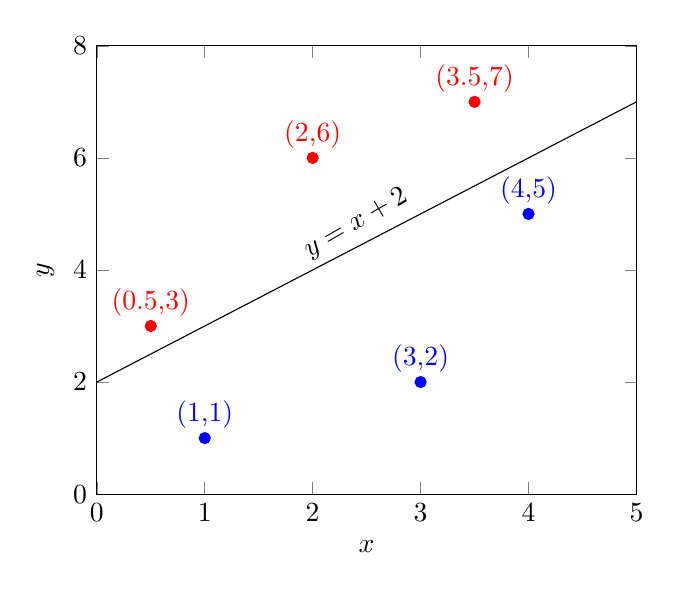
\begin{tikzpicture}
							
							\begin{axis}[xmin = 0, xmax = 5, ymin = 0, ymax = 8, ylabel={$y$ }, xlabel ={$x$},x post scale = 1]
											\addplot[domain = 0:5, samples = 200,black]{x + 2} node[midway,above,rotate=30] {$y = x + 2$};
											% \addplot[domain = 0:2, samples = 200,blue]{1-x};


											\addplot[mark=*, blue] coordinates {(1,1)} node[above] {(1,1)};
											\addplot[mark=*, blue] coordinates {(4,5)} node[above] {(4,5)};
											\addplot[mark=*, blue] coordinates {(3,2)} node[above] {(3,2)};

											\addplot[mark=*, red] coordinates {(2,6)} node[above] {(2,6)};
											\addplot[mark=*, red] coordinates {(0.5,3)} node[above] {(0.5,3)};
											\addplot[mark=*, red] coordinates {(3.5,7)} node[above] {(3.5,7)};

										\end{axis}
							
							\end{tikzpicture}
							\end{center}
							The points in blue have a label of $+1$, and the points in red have a label of 0.

							We can see that the specified line perfectly divides the points \textbf{but misclassifies every single one}. The red points lie above the line, and so satisfy $y > x + 2$ (and so have $\mathcal{P} = 1$), whilst the blue points lie below the line ($\mathcal{P} = 0$).

							The issue is not the separation of the regions, it is in the \textbf{direction} that the comparison operator looks, if our classifier had tested $y < x + 2$ instead of $y > x+2$ then it would work perfectly. 

							However, there is in general no way to know in advance which direction is needed, and so this failed. 

							This is where our extra dimension comes in handy. Consider the dot product $\vec{w} \cdot \tilde{\vec{x}}$ in two dimensions:

							\begin{spalign}
								\vec{w} \cdot \tilde{\vec{x}} & > 0
								\\
								w_0 + w_1 x + w_2 y & > 0
								\\
								w_2 y & > -w_1 c - w_0
							\end{spalign}
							If we let $w_1 = -m$ and $w_0 = -c$ then:
							\begin{spalign}
								w_2 y > m x + c
							\end{spalign}
							This is exactly as we expect. However, if we divide by $w_2$ we need to be careful, and recall how inequality operators (mis)behave when you multiply or divide by negative numbers:
							\begin{spalign}
								w_2 y > mx + c ~~~~ \longrightarrow ~~~ \begin{cases}
									 y > \frac{mx + c}{w_2} & w_2 > 0 
									 \\
									 y < \frac{mx + c}{w_2} & w_2 < 0
								\end{cases}
							\end{spalign}

							We see that the \textit{sign} of $w_2$ changes the direction of the comparison operator. If $w_2$ is negative then we look below the line, and if $w_2$ is positive then we look above it. 

							This is where our extra dimension comes from. Technically speaking, we could get away with simply defining $(m,c)$ and then a direction (either $\pm 1$), but it turns out that if we're going to the trouble of having an extra dimension anyways, then it helps the convergence if we give the line the full freedom to move $w_2$ around as it wants -- this, for instance, allows the line to pivot around smoothly wihtout undergoing drastic changes when the direction changes.

							So why do we need $n+1$ dimensions? Because we don't just need to split the line into two parts, but also assign each part a specific label.

							This is naturally tied in with the idea of the bias, but the bias itself is not the cause, since an alternative formulation which includes a bias term suffers from the same problem!

				\subsection{Training a Perceptron}

						Being able to compute a prediction $\mathcal{P}$ from $\vec{x}$ is all very well and good, but how do we determine what $\vec{w}$ is?

						In order to do that we need to have a \textit{training set} - a series of data points $\vec{x}_i$ which each have their own true label $L_i$.

						The Perceptron training algorithm is very simple:
						\begin{itemize}
							\item Loop through the data, and make a prediction $\mathcal{P}(\vec{x}_i)$.
							\item If $\mathcal{P}_i \neq L_i$ (i.e. the prediction is wrong), update the weights according to:
							$$ \vec{w} \to \vec{w}^\prime  = \vec{w} + r \times(L_i - \mathcal{P}_i ) \tilde{\vec{x}}$$
							\item Repeat until either a set number of loops has completed, or until all predictions are correct.
						\end{itemize}

						Here $r > 0$ is the `learning rate' and determines by how much the weights get updated: small values mean many loops will take to converge (but it won't miss narrow optima), large values mean it will jump around quickly (but might miss the optima).

						\subsubsection{Why does this update formula work?}
						
							If the update formula is being called, then $\mathcal{P}_i \neq L_i$, and we have two options:
							\begin{enumerate}
								\item $L_i = 0$ (and so $\mathcal{P}_i = 1$). This means $\vec{w} \cdot \tilde{\vec{x}}_i > 0$, and so we want $\vec{w}^\prime \cdot \tilde{\vec{x}}_i$ to be \textit{smaller}.
								\item $L_i = 1$ (and so $\mathcal{P}_i = 0$). This means $\vec{w} \cdot \tilde{\vec{x}}_i \leq 0$, and so we want $\vec{w}^\prime \cdot \tilde{\vec{x}}_i$ to be \textit{bigger}.
							\end{enumerate}

							If we compute the new dot product after the weights have been updated:
							\begin{spalign}
								\vec{w}^\prime \cdot \tilde{\vec{x}}_i = \vec{w} \cdot \tilde{\vec{x}}_i + r \left( L_i - \mathcal{P}_i \right) |\tilde{\vec{x}}_i|^2
							\end{spalign}
							By definition, both $r$ and $|\tilde{\vec{x}_i}|^2$ are positive, and so:
							\begin{spalign}
								\vec{w}^\prime \cdot \tilde{\vec{x}}_i &= \vec{w} \cdot \tilde{\vec{x}}_i + \text{positive} \times (L_i - \mathcal{P}_i)
								\\
								& = \vec{w} \cdot \tilde{\vec{x}}_i + \begin{cases} \text{positive} & L_i = 1
									\\
									\text{negative} & L_i = 0\end{cases}
							\end{spalign}

							We can therefore see that he new dot product gets bigger if $L_i = 1$ and gets smaller if $L_i = 0$. This pushes the dot product towards 0, and hence towards the value at which its decision will change.

							This explains why $\tilde{\vec{x}}$ appears in the update formula: it is a vector $\vec{v}$ for which it is guaranteed that $\vec{v} \cdot \tilde{\vec{x}} > 0$, and hence improve the prediction -- we could replace it by any linear scaling of $\tilde{\vec{x}}$ (for instance, $\vec{v} = \frac{1}{|\tilde{\vec{x}}|} \tilde{\vec{x}}$), but it has to point in the same direction.
			\section{Linearity \& Perceptrons}

				One major limitation of Perceptrons is their inherent linearity: by definition they split the $n$ dimensional spaces into 2 parts using a $n-1$ dimensional hyperplane. With our $n+1$ parameters we may have given them the freedom to choose which side to give which labels, but nothing yet gives them the ability to draw a curved line to disentangle data.

				We \textit{can} get around this, however -- all within the framework of a simple perceptron. 
				
				We consider augmenting our input vector with \textit{non-linear combinations of the input features.}

				For instance:
				\begin{equation}
					\begin{pmatrix}
						x \\ y
					\end{pmatrix} \to \begin{pmatrix}
						1 \\ x \\ y \\ x^2 \\ xy \\ y^2
					\end{pmatrix}
				\end{equation}
			
				In doing so we project our input vector into a higher order space (in this case, the 5-dimensional space), and because this projection ocurred in a non-linear fashion, when the Perceptron draws a line through the space and projects it back down into 2D, the result will look like a curved line. 

				This particular choice permits the classification of all possible hyperbolically-separable spaces, instead of just the linearly separable spaces. We can extend the dimensionality even further:
				\begin{equation}
					\begin{pmatrix}
						x \\ y
					\end{pmatrix} \to \begin{pmatrix}
						1 \\ x \\ y \\ x^2 \\ xy \\ y^2 \\ x^3 \\ x^2 y \\ x y^2 \\ y^3 \\ \vdots \\x^{210} y^{100} \\ x^{209} y^{101} \\ \vdots
					\end{pmatrix}
				\end{equation}
				In doing so we leverage the power of Taylor expansions, and can therefore use this to separate \textbf{all possible analytically separable classes}.

				That's right: a single perceptron node can, with suitable modifications, work on arbitrary analytical spaces. Forget what you've been told about the XOR problem!

				\begin{aside}
					This isn't anything new: this is a variation on what is known as the `kernel trick' in SVM terminology, but I rarely see it put into these terms!

					The Kernel Trick varies in that it doesn't require an explicit mapping, relying instead on similarity measures; but it remains the case that for any specified `Kernel Trick' you can decompose it into a non-linear predictor above (doing so is often intractable however, even if theoretically possible).
				\end{aside}

				The problem with this is twofold: it gets complicated \textit{really} fast. As soon as you include terms of suitably high order (I personally had trouble above 8th order), the convergence of your perceptron is absolutely terrible unless you dive in and hold its hand: the higher order terms will flip flop like crazy. Even with $r$ tiny, each update will completely alter your decision boundaries. 

				This is why things like the Kernel Trick exist: they permit this kind of behaviour in a much more controlled fashion, allowing the additional dimensionality and flexibility, without the penalty of accidentally altering $\vec{w}$ by an amount equal to $10^{85}$.

				In short, whilst the Perceptron is, contrary to what you may have heard, capable of dealing with ludicrously non-linear classification tasks, the formulation is poorly suited for them. 
				
				We need something more powerful....maybe some \textit{layers}?

		\chapter{Multi-Layer Perceptrons}

			We saw that, in the case of the non-linear perceptron that, if we project our vector $\vec{x}$ into some high dimensional space, then it was possible for the classifier to then `thread the needle' and draw a decision boundary which was a straight line in the high dimensional space, but a curved shape in the output space. 

			The problem, as we saw, was that this projection had to be manually encoded and resulted in highly unstable behaviour. 
			
			\section{The Naive Perceptron}
				The basic principle of a multi-layer perceptron is that we abstract this projection process into another learnable process: rather than forming our nonlinear vector ourselves, we let the machine learn what would be a good way to manipulate the data -- using a series of individual perceptrons.

				The prediction algorithm then becomes:
				\begin{itemize}
					\item Take our input vector, $\vec{x}$ and pass it into an array of perceptrons. Each perceptron -- called a `node' or a `neuron' then performs a dot product $\vec{w}_i \cdot \tilde{\vec{x}}$. We then collect the results into a new vector $\vec{x}_\text{processed}$
					\item We then repeat this an arbitrary number of times, taking our vector, passing into through an array of neurons, and then collecting the result into a vector, and passing it on to the next `layer' of neurons.
					\item We can then the output of this highly dimensional process as the input to our `decision' node which performs the usual perceptron algorithm.
				\end{itemize}
				A schematic of this kind of perceptron is shown in Fig. \ref{F:Naive}.

				This algorithm is rather simple to code up: it simply requires a way to pass information through the layer. However, if one writes it up a problem will become obvious even without training. 

				If one randomly initialises the weights in all of the nodes and plots the values of the prediction across a range of values -- as is done in figure \ref{F:Linear} -- it becomes very clear that something has gone awry.

				Despite projecting up into our high-dimensional space, \textbf{the decision boundary is still a straight line}! This is despite our projections going up into a 5D space, down into 3D and before going into 1D.

				\begin{figure*}
					\begin{center}
			
					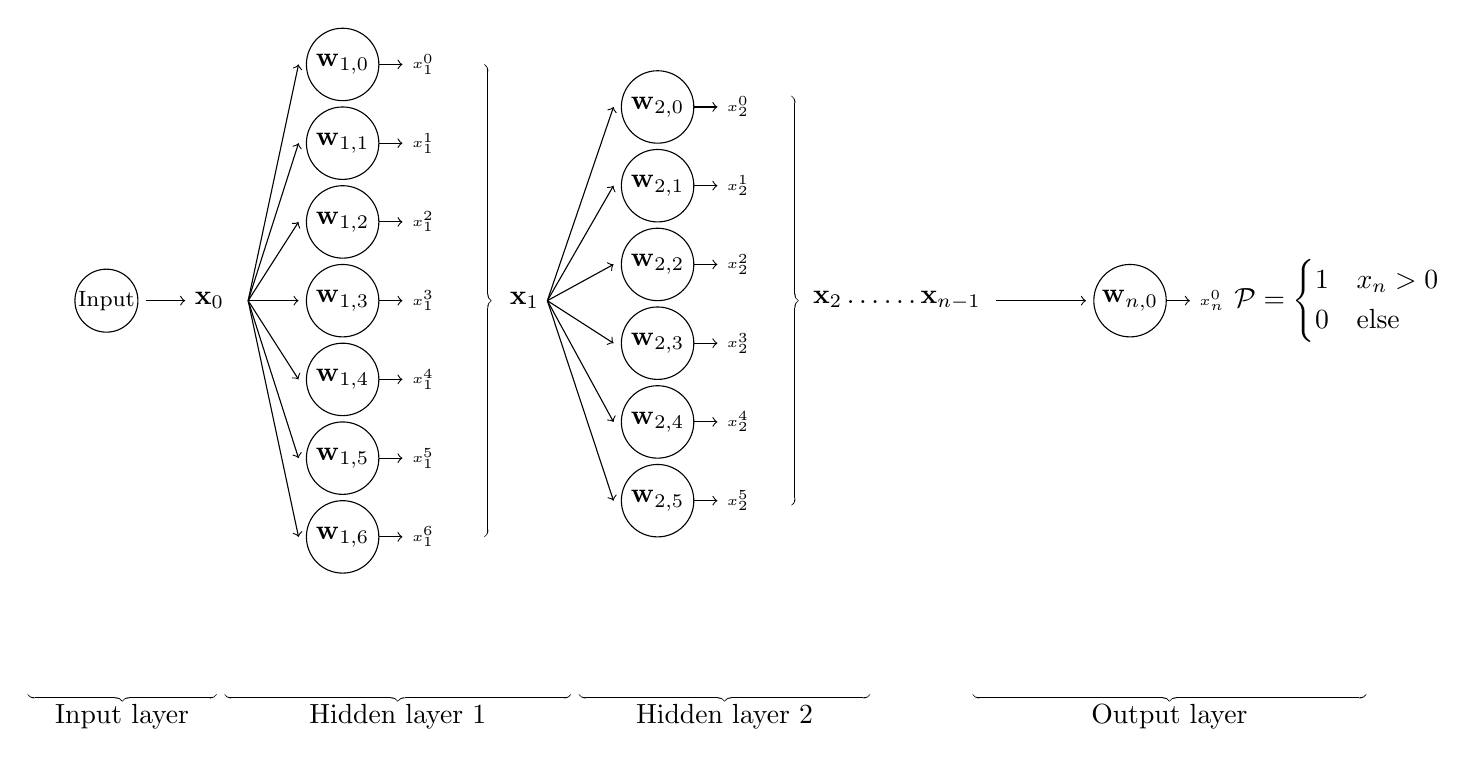
\begin{tikzpicture}
						\draw (0,0) circle (0.4);
						\node at (0,0) {\footnotesize Input};
						\draw[->] (0.5,0)--++(0.5,0);
						% \foreach \i[count=\j from 0] in {2,1,...,-2}
						% {
						% 	\def\r{0.3}
						% 	\def\y{\i/2}
						% 	\def\x{1}
						% 	\draw[->] (0.43,0)--({\x-\r-0.07},\y);
						% 	\draw[fill=white] ({\x-\r},{\y-\r})--({\x+\r},{\y-\r})--({\x+\r},{\y+\r})--({\x-\r},{\y+\r})--cycle;
						% 	\node at (\x,{\y}) {\fontsize{1}{0}\selectfont $[\vec{x}_0]_\j$};
						% }
						\def\baseheight{-5}
						\draw [decorate, decoration = {calligraphic brace}] (1.4,\baseheight) --node[below]{Input layer}  (-1,\baseheight);
						\draw [decorate, decoration = {calligraphic brace}] (5.9,\baseheight) --node[below]{Hidden layer 1}  (1.5,\baseheight);
						\draw [decorate, decoration = {calligraphic brace}] (9.7,\baseheight) --node[below]{Hidden layer 2}  (6,\baseheight);
						\draw [decorate, decoration = {calligraphic brace}] (16,\baseheight) --node[below]{Output layer}  (11,\baseheight);
						% \draw [decorate, decoration = {calligraphic brace}] (1.3,1.2) --  (1.3,-1.2);
						\node[anchor=west] at (1,0) {$\vec{x}_0$};
			
						\foreach \i[count=\j from 0] in {3,2,...,-3}
						{
							\def\r{0.46}
							\def\y{\i}
							\def\x{3}
							\draw[->] (1.8,0)--({\x-\r-0.1},\y);
							\draw (\x,{\y}) circle ({\r});
							\node at (\x,{\y}) { $\vec{w}_{1,\j}$};
							\draw [->] ({\x+\r},{\y})--({\x+\r+0.3},{\y});
							\def\xx{\x+\r+0.3}
							% \draw[fill=white] ({\x-\r},{\y-\r})--({\x+\r},{\y-\r})--({\x+\r},{\y+\r})--({\x-\r},{\y+\r})--cycle;
							\node[anchor=west] at (\xx,{\y}) {\fontsize{1}{0}\selectfont$x_{1}^{\j}$};
						}
						\draw [decorate, decoration = {calligraphic brace}] (4.8,3) --  (4.8,-3);
						
						\node[anchor=west] at (5,0) {$\vec{x}_1$};
			
						\foreach \i[count=\j from 0] in {2,1,0,-1,-2,-3}
						{
							\def\r{0.46}
							\def\y{\i+\r}
							\def\x{7}
							\draw[->] (5.6,0)--({\x-\r-0.1},\y);
							\draw (\x,{\y}) circle ({\r});
							\node at (\x,{\y}) { $\vec{w}_{2,\j}$};
							\draw [->] ({\x+\r},{\y})--({\x+\r+0.3},{\y});
							\def\xx{\x+\r+0.3}
							% \draw[fill=white] ({\x-\r},{\y-\r})--({\x+\r},{\y-\r})--({\x+\r},{\y+\r})--({\x-\r},{\y+\r})--cycle;
							\node[anchor=west] at (\xx,{\y}) {\fontsize{1}{0}\selectfont$x_{2}^{\j}$};
						}
						\draw [decorate, decoration = {calligraphic brace}] (8.7,2.6) --  (8.7,-2.6);
						\node[anchor=west] at (8.85,0) {$\vec{x}_2\hdots\hdots\vec{x}_{n-1}$};
						\foreach \i[count=\j from 0] in {0}
						{
							\def\r{0.46}
							\def\y{\i}
							\def\x{13}
							\draw[->] (11.3,0)--({\x-\r-0.1},\y);
							\draw (\x,{\y}) circle ({\r});
							\node at (\x,{\y}) { $\vec{w}_{n,\j}$};
							\draw [->] ({\x+\r},{\y})--({\x+\r+0.3},{\y});
							\def\xx{\x+\r+0.3}
							% \draw[fill=white] ({\x-\r},{\y-\r})--({\x+\r},{\y-\r})--({\x+\r},{\y+\r})--({\x-\r},{\y+\r})--cycle;
							\node[anchor=west] at (\xx,{\y}) {\fontsize{1}{0}\selectfont$x_{n}^{\j}$};
						}
						% \draw [decorate, decoration = {calligraphic brace}] (15,1) --  (15,-1);
						\node[anchor=west] at (14.2,0) {$\mathcal{P} = \begin{cases} 1 & x_n > 0 \\ 0 &\text{else}\end{cases}$};
					\end{tikzpicture}
					
					\end{center}\caption{A ``Na\"ive MLP'' showing the multiple layers of dot products and collection, before a final perceptron layer.}\label{F:Naive}
				\end{figure*}


				\begin{figure*}
					\newcommand\image[1]
					{
						\includegraphics[width=0.4\linewidth,keepaspectratio=true]{../Presentation/Images/#1}
					}
					\begin{tabular}{cc}
						\image{linear_1} & \image{linear_2} \\ \image{linear_3} & \image{linear_4}
					\end{tabular}
					\caption{The predictions of 4 randomly initialised ``naive MLP''s with dimensionality (5-3-1). The predictions for a 200x200 array of values between (-10,10) are shown. Predictions of label 0 are in red, label 1 in blue.}\label{F:Linear}
				\end{figure*}

				\subsection{What Went Wrong}

					What has gone wrong here is, in fact, rather embarrassing.
					
					If we recall chapter \ref{C:LinearAlgebra}, the definition of matrix multiplication amounted to:
					\begin{spalign}
						W\vec{x} & = \begin{bmatrix}
							\vec{w}_0 \\ \vec{w}_1 \\ \vec{w}_2 \\ \vdots 
						\end{bmatrix} \vec{x}
						\\
						& = \begin{pmatrix}
							\vec{w}_0 \cdot \vec{x} \\ \vec{w}_1 \cdot \vec{x} \\ \vec{w}_2 \cdot \vec{x} \\ \vdots
						\end{pmatrix}
					\end{spalign}
					That is, matrix multiplication is equal to taking the dot product of each row of a matrix with the vector, and then stacking the results into a vector. If we observe Fig \ref{F:Naive} then ``taking the dot product and stacking them into a vector'' is \textit{precisely} what we are doing. 

					Each layer in the network is computing the matrix product with $W_n$, the matrix formed from stacking all of our weights in the $n^\text{th}$ layer into a matrix:
					\begin{equation}
						\vec{x}_n = W_n \tilde{\vec{x}}_{n-1}
					\end{equation}
					Or (if we recall our Affine/augmentation conversation in Chapter \ref{S:Affine}), this is equal to:
					\begin{equation}
						\vec{x}_n = \mathcal{W}_n\vec{x} = W_n^\prime \vec{x} + \vec{b}_n
					\end{equation}				
					Where $W_n = [\vec{b}_n W_n^\prime]$ are the weight/bias components of $W_n$, and $\mathcal{W}_n$ is a general Affine transformation. 
					
					The final output of our network is therefore a stack of these Affine transformations: matrix multiplications plus bias offsets:
					\begin{spalign}
						\vec{x}_n &= \mathcal{W}_n \mathcal{W}_{n-1} \mathcal{W}_{n-2} \cdots \mathcal{W}_2 \mathcal{W}_1 \vec{x}_\text{inputs}
						\\
						& = \vec{b_n} + W_n\left( \vec{b}_{n-1} + W_{n-1} \left( \cdots W_2\left(\vec{b_1} + W_1\vec{x}_\text{inputs}\right) \right)\right)
					\end{spalign}
					Whilst this looks horrible and awful, we recall that affine transforms are associative, which means we can write \textbf{all of this as a single affine transformation} or, in other words 
					\begin{spalign}
						\vec{x}_n & =\mathcal{W}^\prime \vec{x}_\text{input}
						\\
						& = \vec{b}^\prime + W^\prime \vec{x}_\text{input}
					\end{spalign}
					And since our final layer has dimension 1 (a scalar)\dots
					\begin{equation}
						x_n = b + \vec{w} \cdot \vec{x} = \vec{w} \cdot \cec{x}
					\end{equation}
					\textbf{All of this reduces back down into a single perceptron predictor.} All of our layers and increased dimensionality \textbf{did absolutely nothing}. Diddly squat.

					This network is essentially a very long, very convoluted way of computing a single dot product. Well done us. 


			\newpage
			\section{The Feedforward Neural Network}

				OK. Well that didn't go to plan, did it? Those of you familiar with neural network architecture might have thought we were onto a winner, there. 

				What went wrong, however, was that we were attempting to induce non-linearity\footnote{or at least, non-affine-ness, which is a mathematically important distinction, if not a conceptually important one! You may assume I am using affine and linear as essentially synonymous.}...using linear operations. 

				We projected into a higher dimensional space, hoping this would let us draw nice warped lines as straight lines -- but our method of projecting was inherently linear. It was a doomed endeavour from the beginning. 

				Luckily, there is a simple solution to this: \textbf{do something non-linear to the vectors}. 

				It really is as simple as that. Instead of collecting the output of each node into $\vec{x}$ to be converted into $\cec{x}$ and passed onto the next layer of the network, we collect them into a temporary vector $\vec{y}$, and then perform some non-linear operation on that vector - the result of which is then used as $\vec{x}$. This function might vary between each layer, and so we denote it as $\mathcal{F}_n$:
				\begin{equation}
					\vec{y}_n = \mathcal{W}_n \vec{x}_{n-1} ~~~~~~ \vec{x}_n = \mathcal{F}_n(\vec{y}_n)
				\end{equation}
				An example of this kind of function is shown in Fig. \ref{F:Activated}, and it might start to look familiar!
				\begin{figure*}
					\begin{center}
			
					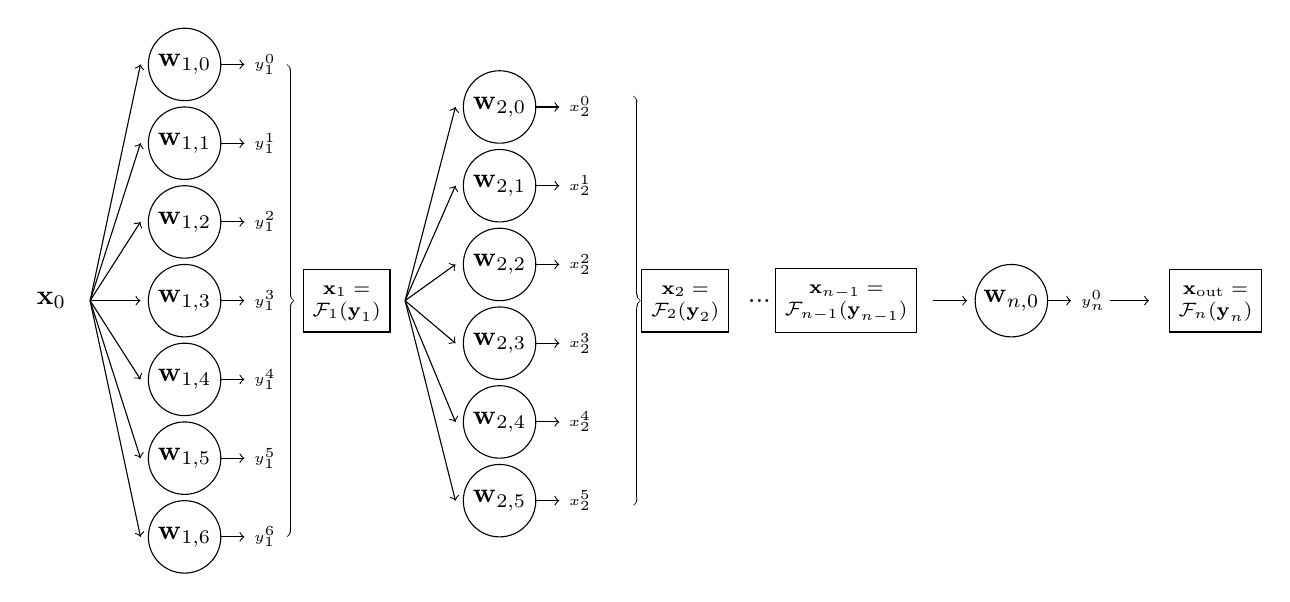
\begin{tikzpicture}
						
						% \foreach \i[count=\j from 0] in {2,1,...,-2}
						% {
						% 	\def\r{0.3}
						% 	\def\y{\i/2}
						% 	\def\x{1}
						% 	\draw[->] (0.43,0)--({\x-\r-0.07},\y);
						% 	\draw[fill=white] ({\x-\r},{\y-\r})--({\x+\r},{\y-\r})--({\x+\r},{\y+\r})--({\x-\r},{\y+\r})--cycle;
						% 	\node at (\x,{\y}) {\fontsize{1}{0}\selectfont $[\vec{x}_0]_\j$};
						% }
						\def\baseheight{-5}
				
						% \draw [decorate, decoration = {calligraphic brace}] (1.3,1.2) --  (1.3,-1.2);
						\node[anchor=west] at (1,0) {$\vec{x}_0$};
			
						\foreach \i[count=\j from 0] in {3,2,...,-3}
						{
							\def\r{0.46}
							\def\y{\i}
							\def\x{3}
							\draw[->] (1.8,0)--({\x-\r-0.1},\y);
							\draw (\x,{\y}) circle ({\r});
							\node at (\x,{\y}) { $\vec{w}_{1,\j}$};
							\draw [->] ({\x+\r},{\y})--({\x+\r+0.3},{\y});
							\def\xx{\x+\r+0.3}
							% \draw[fill=white] ({\x-\r},{\y-\r})--({\x+\r},{\y-\r})--({\x+\r},{\y+\r})--({\x-\r},{\y+\r})--cycle;
							\node[anchor=west] at (\xx,{\y}) {\fontsize{1}{0}\selectfont$y_{1}^{\j}$};
						}
						\draw [decorate, decoration = {calligraphic brace}] (4.3,3) --  (4.3,-3);
						

						\node[rotate=0,anchor=west,draw] at (4.5,0) {\scriptsize $\begin{matrix} \vec{x}_1 = \\\mathcal{F}_1(\vec{y}_1)\end{matrix}$};
			
						\foreach \i[count=\j from 0] in {2,1,0,-1,-2,-3}
						{
							\def\r{0.46}
							\def\y{\i+\r}
							\def\x{7}
							\draw[->] (5.8,0)--({\x-\r-0.1},\y);
							\draw (\x,{\y}) circle ({\r});
							\node at (\x,{\y}) { $\vec{w}_{2,\j}$};
							\draw [->] ({\x+\r},{\y})--({\x+\r+0.3},{\y});
							\def\xx{\x+\r+0.3}
							% \draw[fill=white] ({\x-\r},{\y-\r})--({\x+\r},{\y-\r})--({\x+\r},{\y+\r})--({\x-\r},{\y+\r})--cycle;
							\node[anchor=west] at (\xx,{\y}) {\fontsize{1}{0}\selectfont$x_{2}^{\j}$};
						}
						\draw [decorate, decoration = {calligraphic brace}] (8.7,2.6) --  (8.7,-2.6);
						% \node[anchor=west] at (8.85,0) {$\vec{x}_2\hdots\hdots\vec{x}_{n-1}$};

						\node[rotate=0,anchor=west,draw] at (8.8,0) {\scriptsize $\begin{matrix} \vec{x}_2 = \\\mathcal{F}_2(\vec{y}_2)\end{matrix}$};
						\node at (10.3,0) {...};
						\node[rotate=0,anchor=west,draw] at (10.5,0) {\scriptsize $\begin{matrix} \vec{x}_{n-1} = \\\mathcal{F}_{n-1}(\vec{y}_{n-1})\end{matrix}$};
						\foreach \i[count=\j from 0] in {0}
						{
							\def\r{0.46}
							\def\y{\i}
							\def\x{13.5}
							\draw[->] (12.5,0)--({\x-\r-0.1},\y);
							\draw (\x,{\y}) circle ({\r});
							\node at (\x,{\y}) { $\vec{w}_{n,\j}$};
							\draw [->] ({\x+\r},{\y})--({\x+\r+0.3},{\y});
							\def\xx{\x+\r+0.3}
							% \draw[fill=white] ({\x-\r},{\y-\r})--({\x+\r},{\y-\r})--({\x+\r},{\y+\r})--({\x-\r},{\y+\r})--cycle;
							\node[anchor=west] at (\xx,{\y}) {\fontsize{1}{0}\selectfont$y_{n}^{\j}$};
						}
						\draw [->] (14.75,0)--++(0.5,0);
						\node[rotate=0,anchor=west,draw] at (15.5,0) {\scriptsize $\begin{matrix} \vec{x}_\text{out} = \\\mathcal{F}_{n}(\vec{y}_{n})\end{matrix}$};
						% \draw [decorate, decoration = {calligraphic brace}] (15,1) --  (15,-1);
						% \node[anchor=west] at (14.2,0) {$\mathcal{P} = \begin{cases} 1 & x_n > 0 \\ 0 &\text{else}\end{cases}$};
					\end{tikzpicture}
					
					\end{center}\caption{An ``Activated MLP'' showing the multiple layers of dot products and collection, followed by a non-linear function $\mathcal{F}$.} \label{F:Activated}
				\end{figure*}
				There is practically no limit to what $\mathcal{F}$ can be: all it has to be is \textit{not} be equivalent to an Affine transform, which is a pretty broad scope. 

				\subsection{Activation Functions}

					Perhaps the \textit{easiest} way to come up with a non-linear function is to come up with a nice scalar function and then \textit{do it to each element of the vector}. 

					Generally speaking, so long as the function is anything other than a $f(x) = a x +b$, the result is a nonlinear function:
					\begin{equation}
						\mathcal{F}(\vec{y}) = \begin{pmatrix}
							f(y_0) \\ f(y_1) \\ f(y_2) \\ f(y_3) \\ \vdots \\ f(y_n)
						\end{pmatrix}
					\end{equation}
					When you use a function like this, it can be helpful to think of it as being computed simultaneosly with $y_i$ that is, by the individual nodes themselves. You will therefore commonly see things such as the network depicted in Fig. \ref{F:SepAct}, where this scalar function -- called the `activation function' -- is treated as part of the dot product/node operation.


					\begin{figure*}
						\begin{center}
				
						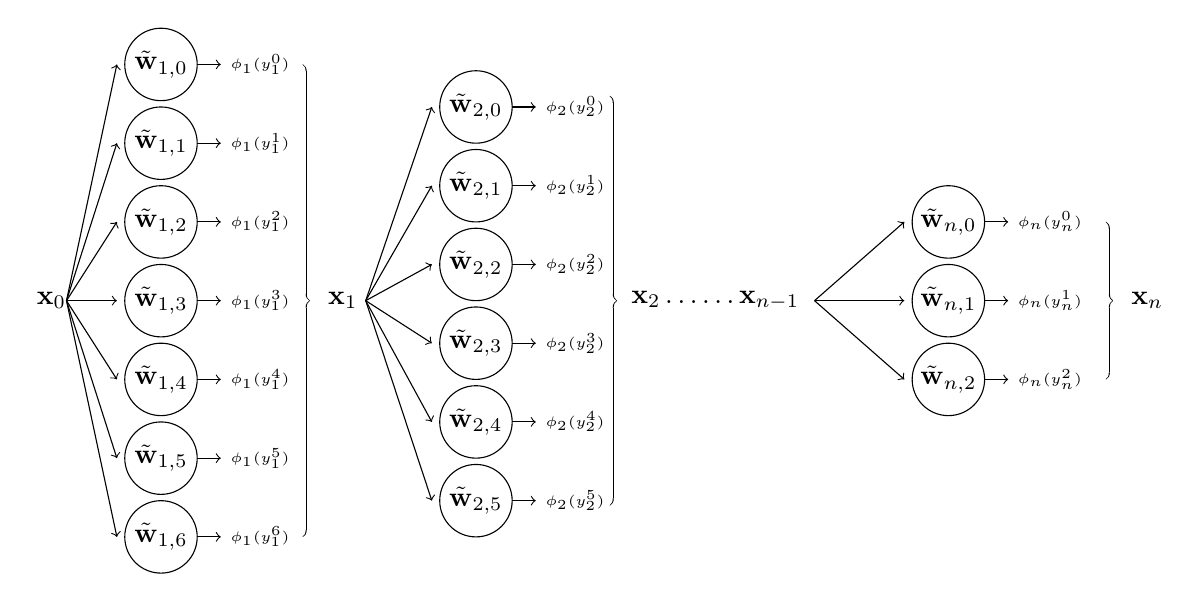
\begin{tikzpicture}
						
						
							\def\baseheight{-5}
							
							\node[anchor=west] at (1.3,0) {$\vec{x}_0$};
				
							\foreach \i[count=\j from 0] in {3,2,...,-3}
							{
								\def\r{0.46}
								\def\y{\i}
								\def\x{3}
								\draw[->] (1.8,0)--({\x-\r-0.1},\y);
								\draw (\x,{\y}) circle ({\r});
								\node at (\x,{\y}) { $\cec{w}_{1,\j}$};
								\draw [->] ({\x+\r},{\y})--({\x+\r+0.3},{\y});
								\def\xx{\x+\r+0.3}
								% \draw[fill=white] ({\x-\r},{\y-\r})--({\x+\r},{\y-\r})--({\x+\r},{\y+\r})--({\x-\r},{\y+\r})--cycle;
								\node[anchor=west] at (\xx,{\y}) {\fontsize{1}{0}\selectfont$\phi_{1}(y_{1}^{\j})$};
							}
							\draw [decorate, decoration = {calligraphic brace}] (4.8,3) --  (4.8,-3);
							
							\node[anchor=west] at (5,0) {$\vec{x}_1$};
				
							\foreach \i[count=\j from 0] in {2,1,0,-1,-2,-3}
							{
								\def\r{0.46}
								\def\y{\i+\r}
								\def\x{7}
								\draw[->] (5.6,0)--({\x-\r-0.1},\y);
								\draw (\x,{\y}) circle ({\r});
								\node at (\x,{\y}) { $\cec{w}_{2,\j}$};
								\draw [->] ({\x+\r},{\y})--({\x+\r+0.3},{\y});
								\def\xx{\x+\r+0.3}
								% \draw[fill=white] ({\x-\r},{\y-\r})--({\x+\r},{\y-\r})--({\x+\r},{\y+\r})--({\x-\r},{\y+\r})--cycle;
								\node[anchor=west] at (\xx,{\y}) {\fontsize{1}{0}\selectfont$\phi_{2}(y_{2}^{\j})$};
							}
							\draw [decorate, decoration = {calligraphic brace}] (8.7,2.6) --  (8.7,-2.6);
							\node[anchor=west] at (8.85,0) {$\vec{x}_2\hdots\hdots\vec{x}_{n-1}$};
							\foreach \i[count=\j from 0] in {1,0,-1}
							{
								\def\r{0.46}
								\def\y{\i}
								\def\x{13}
								\draw[->] (11.3,0)--({\x-\r-0.1},\y);
								\draw (\x,{\y}) circle ({\r});
								\node at (\x,{\y}) { $\cec{w}_{n,\j}$};
								\draw [->] ({\x+\r},{\y})--({\x+\r+0.3},{\y});
								\def\xx{\x+\r+0.3}
								% \draw[fill=white] ({\x-\r},{\y-\r})--({\x+\r},{\y-\r})--({\x+\r},{\y+\r})--({\x-\r},{\y+\r})--cycle;
								\node[anchor=west] at (\xx,{\y}) {\fontsize{1}{0}\selectfont$\phi_{n}(y_{n}^{\j})$};
							}
							\draw [decorate, decoration = {calligraphic brace}] (15,1) --  (15,-1);
							\node[anchor=west] at (15.2,0) {$\vec{x}_{n}$};
						\end{tikzpicture}
						
						\end{center}\caption{An activated MLP where the activation function is computed with the node, as a scalar function $\phi_i(x)$.}\label{F:SepAct}
					\end{figure*}

				\subsection{Non-Separable Activation Functions}

					Although per-node activation functions were biologically motivated by comparison with neurons, it is not necessary to consider them an inherent property of the nodes themselves. 

					In fact, it is often useful to consider more general functions $\mathcal{F}$, where it is proper to think of them as happening as part of the \textit{layer}: the nodes compute $y_i$ which the layer then gathers into $\vec{y}$ and the operation can only be performed once $\vec{y}$ is fully specified. 

					An example of a commonly used non-separable layer-activation function is the `Softmax' function:
					\begin{equation}
						\text{softmax}(\vec{x}) = \frac{1}{\sum_i \exp(x_i)} \begin{pmatrix}
							\exp(x_0) \\ \exp(x_1) \\ \exp(x_2) \\ \vdots
						\end{pmatrix}
					\end{equation}
					This function is used to convert arbitrary vectors $\vec{x}$ into meaningful probability mass arrays: the elements of $\vec{y} = \text{softmax}(\vec{x})$ sum to one and are all between 0 and 1. This layer is often used as the output for one-hot-encoding classifiers, as well as statistically motivated tasks. 

					It is not possible to compute this function on the nodes (without a complex series of nodes-connected-to-nodes-in-their-own-layer, which gets tiresome), because you cannot perform the division without knowing the state of all of the other nodes in the layer.

					Other common non-separable functions include the various pooling and max-ing layers common in CNNs. 

					For our current purposes, it suffices merely to note that, \textit{in general} the function $\mathcal{F}$ is a per-layer function of arbitrary complexity. However, for the majority of practical purposes it is easiest to use per-node scalar activation functions.

				\subsection{The Proof is in the Pudding}

				\begin{figure*}
					\newcommand\image[1]
					{
						\includegraphics[width=0.4\linewidth,keepaspectratio=true]{../Presentation/Images/#1}
					}
					\begin{tabular}{cc}
						\image{nonlinear_1} & \image{nonlinear_2} \\ \image{nonlinear_3} & \image{nonlinear_4}
					\end{tabular}
					\caption{As in Fig. \ref{F:Linear}, but using Sigmoid activation functions instead of linear. The resulting curved lines demonstrate the effectiveness of the method.}\label{F:NonLinear}
				\end{figure*}
					We now implement a common activation function, the Sigmoid (also known as logit)
					\begin{equation}
						\sigma(x) = \frac{1}{1 + \exp(-x)}
					\end{equation}
					This starts at $\sigma = 0$ at $x \ll 0$, and then increases up to $\sigma = 1$ at $x \gg 0$ with a period of linearity around $x \approx 0$. 

					The results of a randomly initialised (5-3-1) function with Sigmoid activation on the hidden layers and a Perceptron classifier on the final layer are shown in Fig. \ref{F:NonLinear}. Unlike the plots of the identical network with linear activation functions (Fig. \ref{F:Linear}) we see that our straight classification boundaries have been replaced by appropriately non-linear ones: we are ready to begin machine learning in earnest!
					
				\subsection{In Defence of Linear Activation Functions}

					It is tempting to think, given all that we have discovered, that the linear activation function $\mathcal{F}(\vec{x}) = \vec{x}$ will never see the light of day.

					This is in fact wildly incorrect. 

					Almost all\footnote{In the \href{https://en.wikipedia.org/wiki/Almost_all}{mathematical sense}, since the space of classification functions is of a lower cardinality than the space of even arbitrary scalar functions, let alone arbitrary functions on $\mathbb{R}^n$.} neural networks have a linear activation function as their final layer. 

					This is because neural networks can be used to approximate \textit{any} function, not just perform classification. If the value of this function is unbounded (i.e. it's not a probability you know should be $0\leq p \leq 1$), then the linear activation function is needed. So long as you have non-linear activation functions within the hidden layers, the output layer being non-linear is of no consequence. 

					I wrote this section after I saw online\footnote{It was reddit. Of course it was reddit} some people arguing that the linear activation function `should never have been coded', which is, of course, dumb.


			\section{Universal Approximation}

				One of the most important properties about a FNN in the way that we have constructed them is that they are \textbf{Universal Approximators}: they are able to model arbitrary functions.

				The Cybenko statement is as follows:

				{\centering \it A FNN with a single hidden layer of infinite width and possessing the Sigmoid activation function can approximate any function}.

				This argument has since been generalised to networks of arbitrary depth, non-sigmoid activation functions, and non-infinite networks. 

				In short: for any conceivable function $f: \mathbb{R}^n \to \mathbb{R}^m$ there is \textit{some} neural network architecture which can replicate it. It does not matter how complex the function is, or what might need to be done to compute it `properly': a FNN of sufficient size can compute it.

				The catch, naturally is twofold:
				\begin{itemize}
					\item There is very little information (\textit{a priori}) about what `sufficient size' is.
					\item These proofs are non-constructive: they tell you a network exists, but give no indication on how to go about constructing it.
				\end{itemize}

				In short: we know that, for every single problem, there exists an FNN which can solve it. But how to go about making that network, or how many trillions of nodes it might need, is left as an exercise to the reader. 

				The difficulty is not the theory, it's in the execution.

				
				

		\chapter{Training an MLP}

			Training an MLP is a fiddly business: the mathematics is actually rather simple (it is merely a recurrence relation on the chain rule) -- the difficulty is merely one of ensuring all the right parts end up in the right places. 

			\section{Setting the Scene}
				The first thing we have to realise is that the simple formula of the Perceptron update formula will no longer work. We will need to tackle this as an \textit{optimisation problem}. We therefore move away from a binary `yes/no' output and into a continuous output.

				In the case of a single-variable classifier, we might use a sigmoid as our final layer neuron (or, in the case of one-hot encoding, a series of them). If we are instead focusing on approximating an arbitrary function, then a linear activation function will suffice. 

				Whichever way we look at it, the output of our network is now a continuous vector $\vec{x}$. We might choose to post-process this into a binary answer (i.e. a classification probability $>0.5$ can be converted into a `yes' and $<0.5$ into a no), but the network itself will utilise continuous outputs. 

				With a continuous output, we can then assign a \textit{cost function}, $C(\vec{x}_\text{output})$. This cost function (also known as a loss function) should be a differentiable function of the prediction value and, as such, is a function of the current network state. 

				A well-behaved cost function $C(\vec{x})$ has the following behaviours:
				\begin{enumerate}
					\item $\pdiv{C}{\vec{x}}$ exists and is computable. 
					\item $C(\vec{x})$ is small when the network prediction is close to the `ground truth', $\vec{y}_\text{truth}$. We may write $C = C(\vec{x} | \vec{y})$
					\item It is large when the prediction is far away.   
				\end{enumerate}

				In this sense, $C$ measures the overall performance of the network. The following score can be assigned to a `training set' of data $(\vec{d}_i)$ where the expected output of the network is known $(\vec{y}_i)$ is known:
				\begin{equation}
					\mathcal{L} = \sum_{\text{data $q$ in set}} C\left( \mathcal{P}(\vec{d}_q | \vec{y}_q) \right)
				\end{equation}
				This function, $\mathcal{L}$ is a function therefore of the training set and of the state of the network, which is determined by the weights:
				\begin{equation}
					\mathcal{L} = \mathcal{L}\left(\{ \vec{w} \}\right)
				\end{equation}

				The task of training the network is therefore equivalent to finding the set of $\{\vec{w}\}$ which minimise the value of $\mathcal{L}$. If we can find these values, we have found the network configuration which best approximates our input function. 

				We recall that the optima of a function are found whenever the derivatives are zero. If $\vec{w}_\ell^i$ is the weights associated with the $i^\text{th}$ node in the $\ell^\text{th}$ layer, then we need to find the point where:
				\begin{equation}
					\pdiv{\mathcal{L}}{\vec{w}_\ell^i} = 0
				\end{equation}
				We must then simultaneously solve this equation for every node in the set. \textbf{This is not analytically possible}. We must therefore resort to the methods of numerical solutions to differential equations, as discussed in Chapter \ref{C:Optimisation}.

				In the case of Newton's gradient descent, for instance, we simply need to be able to iterate over the following equation:
				\begin{spalign}
					\vec{w}_\ell^i \to \vec{w}_\ell^i - \frac{\alpha}{|\vec{d}_\ell^i|}\vec{d}_\ell^i
					\\
					\vec{d}_\ell^i = \pdiv{\mathcal{L}}{\vec{w}_\ell^i}
				\end{spalign}
				The negative sign here is because we are trying to \textit{minimise} our cost function. We could define our cost function to be `large when good' and `small when bad', in which case we would use a $+$ and be maximising. 

				Our goal is now clear: we must find a way to compute these gradients.
				
				This will be a gross task, but the end result is surprisingly tractable.


			\section{Notational Clarification}

				The complexity in this task is one of notation and exploding dimensionality. For that reason, it is important to make sure we are clear about our notation. We recall the distinction between $\vec{x}$, $\cec{x}$ and $\vec{y}$:


				\begin{equation}
					{y}_i^j = \vec{w}_i^j \cdot \tilde{\vec{x}}_{i-1} ~~~~~ \vec{y}_i = \begin{pmatrix}
						y_i^1 \\ y_i^2 \\ y_i^3 \\ y_i^4 \\ \vdots 
					\end{pmatrix}~~~~~~\Longleftrightarrow~~~\vec{y}_i = W_i \cec{x}_{i-1}
				\end{equation}
				That is, ${y}_i^j$ is the \textit{unactivated result} which comes out of node $j$ in layer $i$, and which can be packaged into the vector $\vec{y}_i$; the \textit{unactivated vector} associated with layer $i$.

			Each layer\footnote{Recall that, properly speaking, it is the layer which does the activation. The nodes only do it in the case of simple separable functions} then performs an activation transformation, and we then augment the vector into a higher-dimension (to incorporate the bias):
			\begin{equation}
				\vec{x}_i = \mathcal{A}_i(\vec{y}_i) ~~~~~~~ \tilde{\vec{x}}_i = \begin{bmatrix} 1 \\\mathcal{A}_i(\vec{y}_i)\end{bmatrix}
			\end{equation}
			If this is a separable transform, then it can be written as:
			\begin{equation}
				\tilde{\vec{x}_i} = \begin{pmatrix}
					1 \\ a_i\left( y_i^1\right) \\ a_i\left( y_i^2\right) \\ a_i\left( y_i^3\right)\\ a_i\left( y_i^4\right) \\ \vdots 
				\end{pmatrix}
			\end{equation}
			
			The problem is therefore simple enough to state. The issue is that our cost function is a horrible series of these functions. Taking the derivative is going to be wildly unpleasant. 
		% 	\begin{float}
		% 	For a simple 3-layer network, the problem looks like this:
			\newcommand\afunc[2]
			{
				\mathcal{A}_{#1}\left(\begin{matrix}\vec{w}^1_{#1} \cdot#2 \\ \vec{w}^2_{#1} \cdot#2 \\  \vec{w}^3_{#1} \cdot#2  \\ \vdots \end{matrix} \right)
			}
		% 	\begin{equation}
		% 		\mathcal{P}(\vec{d}_\text{input}) =  \afunc{3}{\afunc{2}{{\afunc{1}{\vec{d}_\text{input}}}}}
		% 	\end{equation}
		% \end{float}



		\section{The Cost Function}


			The Cost function associated with the network is something which is \textbf{minimised} at when the network is performing well, and \textbf{minimised} when it is performing badly. 

			It will be significantly easier (but not actually a requirement) if our cost function is linear in the data, that is, it can be written as:
			\begin{equation}
				\mathcal{L}(\{\vec{d}\}) = \sum_q C(\vec{d}) ~~~~\Longleftrightarrow \pdiv{\mathcal{L}}{\vec{w}} = \sum_q \pdiv{C_q}{\vec{w}}
			\end{equation}
			If we can find the derivative as a function of a single input data, then we simply need to sum the derivatives over all the input data, and we're good to go. 
			
			We will assume that all of our cost functions will take this form, and so $\pdiv{C}{\vec{w}}$ is our primary goal.


			A decent first guess at the cost function would be the least squares function:
			\begin{spalign}
				C(\vec{d}|\vec{\ell}) & = \left(\mathcal{P}(\vec{d}) - \vec{\ell}\right)^2  
				\\
				& = \left(\mathcal{P}(\vec{d}) - \vec{\ell}\right) \cdot \left(\mathcal{P}(\vec{d})- \vec{\ell}\right)
			\end{spalign}
			Here $\mathcal{P}$ is the output of our network (the final output vector), and $\vec{\ell}$ is the label of that data. If our network outputs a scalar, then $\vec{\ell} \to \ell$ and we lose the dot product.

	
			Other cost functions are possible -- and are discussed in detail in section \ref{S:CostFuncs}

		\section{Backpropagation}

			To compute the set of gradients $\left\{\pdiv{C}{\vec{w}_i^j} \right\}$ will, in general, require manual computation of every single one of these multidimensional derivatives.

			Luckily, there is an easier way. 

			The single most important equation we will be using is this chain rule equation, which notes that:
			\begin{spalign}
				\pdiv{C_i}{\vec{w}_i^j} & = \pdiv{C_i}{y_i^j} \pdiv{y_i^j}{\vec{w}_i^j} 
				\\
				& \left( \text{recall } y_i^j = \vec{w}_i^j \cdot \tilde{\vec{x}}_{i-1} \right)
				\\
				& = \pdiv{C_i}{y_i^j} \tilde{\vec{x}}_{i-1}
			\end{spalign}
			\textbf{This is why I suggested the route of augmenting vectors rather than adding the bias manually -- it makes your gradients trivially easy to compute as a whole, rather than having to do the bias separately!}


			\subsection{The Output Layer}

				The output layer is the easiest to compute gradients for, because they do not have a knockon effect on the rest of the network in the way that the hidden layers do.

					We recall that, by definition, $\mathcal{P} = \mathcal{A}(\vec{y_{N}})$, so we merely need to compute
				\begin{spalign}
					\pdiv{C_q}{y_N^i} & = \pdiv{C_q}{p_i} \times \pdiv{C_q}{y_N^i}
					\\
					& = \pdiv{C_q}{p_i} \pdiv{}{y_N^i} a(y_N^i)
				\end{spalign}
			We assume that (since we chose it) if $a_N(x)$ is the activation function of the $N^\text{th}$ layer, then we know that $d_N(x) = \pdiv{a_N}{x}$ is its derivative. We can then write:
			\begin{spalign}
				\pdiv{C_q}{y_N^i} & = \pdiv{C_q}{p_i} \times d_N(y_N^i)
			\end{spalign}

			This means that:
			\begin{spalign}
				\pdiv{C_q}{\vec{w}_\ell^i} = d_N(y_N^i)\pdiv{C_q}{p_i} \cec{x}_{N-1}
			\end{spalign}

			If we use the least squares cost function, then:
			\begin{spalign}
				\pdiv{C_q}{\vec{w}_\ell^i} = d_N(y_N^i) \times \left( p_q^i - \ell_q^i\right) \cec{x}_{N-1}
			\end{spalign}


				
			This is easy to compute \& calculate. It is the product of the activation function's derivative (something we should write when we write the node's activation function itself), the difference between the $i^\text{th}$ element of the prediction vector, $p_q^i$ and it's associated `true label' $\ell_q^i$, and the output of the lower layer vector, $\cec{x}$. 
			
			
			One layer down, an unknown number to go....

			\subsection{The Hidden Layers}
			The next layer, down, however, can be trivially computed from the chain rule. Since the output from layer $p$, $\vec{y}_p$ is only directly used by the layer $p+1$, we can write:
			\begin{equation}
				\pdiv{C_q}{y_p^i} = \sum_{\text{nodes $j$ in $p+1$ layer}} \pdiv{y_{p+1}^j}{y_p^i} \pdiv{C_q}{y_{p+1}^j}
			\end{equation}
			That is, the derivative with respect to the $y$ in layer $p$ is equal to (the sum of) the way in which $y_{p+1}$ affects $C_q$, multiplied by the way in which $y_p$ affects $y_{p+1}$. 

			This seems relatively horrible to write out in mathematics, but we're almost there. 

			The final step is to write $\pdiv{y_{p+1}}{y_p}$ in terms of known variables. We recall that:
			\begin{equation}
				y^j_{p+1} = \vec{w}_{p+1}^j \cdot \begin{bmatrix} 1 \\ a_{p+1}(y_p^1) \\ a_{p+1}(y_p^2) \\ \vdots \end{bmatrix}
			\end{equation}
			Therefore:
			\begin{spalign}
				\pdiv{y^j_{p+1}}{y_p^i} &= \left[ \vec{w}_{p+1}^j \right]_{i+1} \div{}{y_{p}^j} a_{p+1}(y_p^i)
				\\
				& = \left[ \vec{w}_{p+1}^j \right]_{i+1} d_{p+1}(y_p^i)
			\end{spalign}
			\textbf{Note that the index of $[\vec{w}]$ is offset by one: $i+1$ not $i$. This is because of the bias term which sits at the first index of $\vec{w}$.}

			
			\subsection{Putting it All Together}

				This is a lot of maths. The upside is that it is relatively trivial to actually \textit{implement} within the neural network. 

				In order to compute the gradients, we have:
				\begin{equation}
					\pdiv{C_q}{y_\ell^i} = \begin{cases} \pdiv{C_q}{P_q^i} \times d_N(y_N^i) & \text{ if $\ell = N-1$}
					\\
					d_\ell(y_\ell^i) \sum_{j}  \left[ \vec{w}_{\ell+1}^j \right]_{i+1} \pdiv{C_q}{y_{\ell+1}^j}
					
					\end{cases}
				\end{equation}
				Where $\pdiv{C_q}{P_q^i}$ is the derivative of your chosen cost function, and $d_N(y)$ is the derivative of the $N^\text{th}$ layer's activation function. Having computed all of these values, it is therefore trivial to find:
				\begin{equation}
					\pdiv{C_q}{\vec{w}_\ell^i} = \pdiv{C_q}{y_\ell^i} \tilde{\vec{x}}_{\ell-1}
				\end{equation}

			\subsubsection{What on Earth just happened?}
				This seems imposing, so it is worth reiterating what is happening.
				\begin{itemize}
					\item We first start by passing the information \textit{forward} through the network, in order to compute our values of $\vec{y}$, and $\tilde{\vec{x}}$ since we need these to compute the gradients.
					\item We then move to the back of the network by first computing how the score changes if the prediction changes. This is $\pdiv{C_q}{P_q^i}$: it tells us how the score $(C)$ of the $q^\text{th}$ datapoint changes when we tweak the value of $P$, the prediction. 
					\item The final layer of the network (the one which makes $P$) then uses this information to work out how $P$ changes when it tweaks its unactivated values, $\vec{y}$. It then uses this to work out how the score $C$ changes when $y$ is tweaked: this is $\pdiv{C}{y_N}$. 
					\item Th next layer down then works out how much $\vec{y}_N$ changes when the layer $N-1$ tweaks \textit{its} unactivated values. The rate at which $C$ changes in response is just the product of the higher layer's gradients times these internal tweak values, giving us $\pdiv{C}{y_{N-1}}$
					\item Then we repeat through the network, each time using the upper layer's gradient to compute the gradient of the next layer. 
					\item When we reach the first layer, we are almost done.
					\item We then go back through the network and use $\pdiv{C}{y}$ to compute $\pdiv{\mathcal{L}}{\vec{w}}$ -- this is a simple multiplication!
				\end{itemize}
		\chapter{Training Considerations}

			I won't spend too much time talking about things here because entire tomes have been written about them elsewhere, this will be a brief overview of some major themes.


			\section{Modified Cost Functions}\label{S:CostFuncs}

				The choice of Cost (or Loss) function is an important one, because it specifies the kinds of behaviours that you wish to encourage in the model, and -- perhaps most importantly -- the kinds of scales of errors that you are willing to tolerate. 

				For example, the least squares error does a decent enough job for fitting functions, but if your prediction value is to be interpreted as a probability, then it exhibits some undesirable behaviour. 
				
				Consider the case where a value in your training set \textit{should} have a predicted probability of 0.25: the last squares assigns the same penalty to prediction of 0.001 as it does to a prediction of 0.5001.

				However, in the realm of probability, 0.25 and 0.5 are rather `close' -- they both describe an event which is plausible; whereas 0.001 describes an event which is (almost) impossible. Although the absolute difference in probabilities is the same, the meaning behind these is very different. As a statistician I am not (particularly) worried if my model regularly predicts something as being 10\% more common than it should be: I \textit{am} worried if it regularly predicts that something common is in fact highly implausible.

				My model should react far more strongly to a $0.25 \to 0.001$ error than it should to a $0.25 \to 0.5$ error, and the least squares method simply does not do that!

				If we wish to encourage the model to consider the scale as important, then a cost function on the Logarithms is more appropriate. If we go back to an true/false labelled dataset, then:
				\begin{equation}
					C = \begin{cases} \log(\mathcal{P}(\vec{d})) & \ell = 1
						\\
						\log(1 - \mathcal{P}(\vec{d})) & \ell = 0
					\end{cases} ~~~~~~~~\text{and} ~~~~~~ \pdiv{C}{\mathcal{P}} = \begin{cases} \frac{1}{\mathcal{{P}}} & \ell = 1
						\\
						\frac{-1}{1 - \mathcal{P}} & \ell = 0\end{cases}
				\end{equation}


				One popular one is (motivated by statistics) to assume a one-hot encoding, where $\vec{\ell} = (0,0,\hdots,1,\hdots,0)$ is a vector of zeros, except at the index associated with its classification. This lends itself to a `cross entropy' cost function which is (if the output vector is interpreted as a probability) merely the log-posterior of the predictor:
				\begin{equation}
					C(\vec{d}|\vec{\ell}) = \sum_i \ell_i \log(p_i)~~~~~~ p_i = \left[ \mathcal{P}(\vec{d}) \right]_i
				\end{equation} 
				When writing this, one has to make special note that $0 \times \log(0) = 0$, because otherwise your computer will cry.

			\section{Degradation \& Convergence}

				It seems intuitive that simply shouting `MORE!' and adding more, bigger layers into a network will improve the accuracy of the prediction. After all, the Universality Theorems state that, with sufficient size, we can model any function. 

				Why don't I want to make my model as large as possible?

				Intuitively it would seem that this could \textit{only} make our results better. Empirically, however, it becomes obvious that this does not result in the desired improvements -- in fact, making networks \textit{larger} often makes them \textit{worse}.
				
				There are two slightly different ways to understand this counterintuitive result, which is known as the Degradation Problem.

				\subsection{Convergence, Gradients}

					A fundamental problem of numerical optimisation is that it is never possible to prove that any given location is a global maximum; and (even worse), given the finite resolution of numerical methods, it is actually impossible to prove that a given location is even an optimum, and not just an area of non-zero-but-below-computational-$\epsilon$-gradient.

					Simply put: you never know if your model has converged, and even if you did, you never know if your model has found a global solution. 

					These problems exist in all numerical optimisation problems (where it is often sufficient to get `close enough'). The problem with Neural Networks is that as you add layers, you also increase the dimensionality of the optimisation space. 

					This induces two problems; it increase the (potential) number of local optima\footnote{And recall, we \textit{know} there are multiple global optima which produce the same output, since there are multiple functions which produce the same output over the training set data -- this does not even account for the number of local optima!}, but also makes us susceptible to the Vanishing Gradients Problem. 

					In a network of sigmoids where the gradient is bounded between $[-1,1]$, the tendency of the chain rule is to cause the gradient to decrease the deeper into the model one goes; and when the model gets sufficiently large, the gradient becomes so small that the optimiser is unable to move the parameters. An opposite problem -- the Exploding Gradients Problem -- can also happen, in which case the optimiser moves, but in a chaotic, haphazard fashion which can cause overflows and numerical instability. 

				\subsection{The Identity Problem}

					Consider a network of $N$ layers, which functions perfectly, mapping input $\vec{x}$ to output $\vec{y}$. We now add this network as the `head' of a larger model with $M$ layers. 

					It would seem, intuitively, that this network should still be able to work perfectly since all the $M$-layer network needs to do is perform the mapping $\vec{x} \to \vec{x}$ and the perfect $N$-layer network will function as expected. 

					The problem, as it turns out, is that this mapping (the identity mapping) is actually really quite difficult for a neural network to do. 

					The issue is rather simple. This is a linear operation -- the simplest possible linear operation, in fact.

					\textbf{But we went to quite some effort to grant our Neural Networks non-linear properties.}
					
					Our construction of Neural Networks was designed in such a way as to make this incredibly simple operation surprisingly difficult. 

					Therefore, adding layers past the point of `being enough' can actually lead to a degradation in performance, unless you go to efforts to construct your network to permit linear operations in certain cases -- ResNets are an example where the input vector $\vec{x}$ gets passed through the network on `free connections'. The intermediary layers are therefore modelling the function $f(x) - x$. If the model thinks that $\vec{x}$ is better than a non-linear mapping then it can just set $\vec{w} = 0$ (for a ReLu network), such that $f(x) -x = 0 \to f(x) = x$.


					These `highway paths' are an integral part of modern architectures such as Transformers and enable networks to grow much larger than a na\"ive FNN can plausibly permit.



			\section{Interpolation}

				The Universality theorem -- which, to recap, guarantees that a FNN of sufficient size is able to model any possible function -- is brilliant, and is what enables modern Machine Learning as a field of study. 

				However, it has one major, major downside: the value of the optimal set of weights, $\{\vec{w}\}$ is conditioned on the input data. 

				That is, you do not actually train your network on a function (which usually has an infinite continuum of input and output values), but on a finite sample of points. The Universality Theorem does not guarantee that the network will fit \textbf{the} function which provides your sample, but \textbf{any} function which is capable of producing those same outputs. 

				For example, consider a network which is trained to predict function values based on some sample points. For the given input data, the Universality Theorem talls us absolutely nothing about which function a Neural Network will prefer -- even if one seems more evidently `correct' than the other to us. 

				\begin{center}
					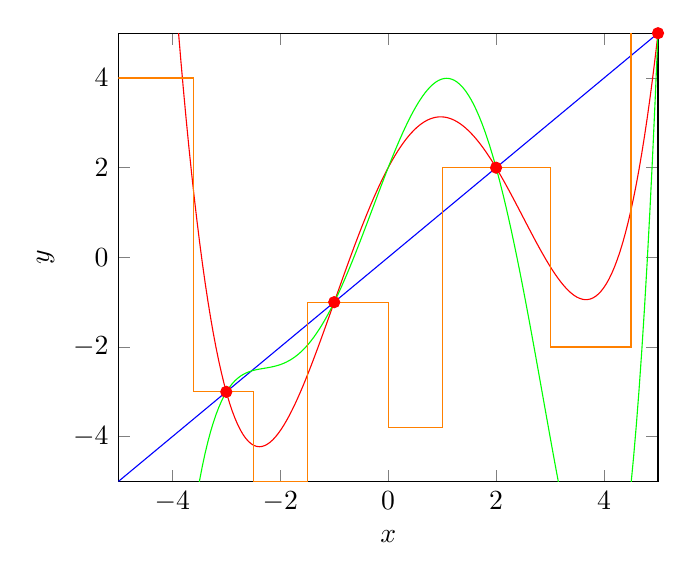
\begin{tikzpicture}
					
					\begin{axis}[xmin = -5, xmax = 5, ymin = -5, ymax = 5, ylabel={$y$ }, xlabel ={$x$},x post scale = 1]
									\addplot[domain = -5:5, samples = 200,blue]{x};
									\addplot[domain = -5:5, samples = 200,red]{0.06666 * x^4 - 0.2*x^3 - x^2 + 2.2666*x +2};
									\addplot[domain = -5:5, samples = 200,green]{2.0 + 3.06*x^1 - 0.499*x^2 - 0.596*x^3 - 0.0125*x^4 + 0.0264*x^5};
									% \addplot[domain = -5:5, samples = 200,blue]{2.0 + 3.53*x^1 -1 0.356*x^2 -1 0.933*x^3 + 0.0191*x^4 + 0.058*x^5 -1 0.00527*x^6};
									% \addplot[domain = 0:2, samples = 200,blue]{1-x};

									\addplot+[const plot, no marks, orange] coordinates {(-5,4)  (-3.6,-3) (-2.5,-5) (-1.5,-1) (0,-3.8) (1,2) (3,-2) (4.5,5)};


									 \addplot[mark=*, red] coordinates {(-1,-1)};
									 \addplot[mark=*, red] coordinates {(-3,-3)};
									 \addplot[mark=*, red] coordinates {(2,2)};
									 \addplot[mark=*, red] coordinates {(5,5)};
									%  \addplot[domain = -1:1, samples=2, orange, ultra thick]{0};
									%  \addplot[mark=*, orange] coordinates {(0,0)};
								\end{axis}
					
					\end{tikzpicture}
					\end{center}

					All of these functions predict with 100\% accuracy the value of the provided training points, but give wildly divergent values when we ask for predictions outside the training set.

					In short, we are making the same assessment that we make whenever we perform regression and interpolation: we hope that our knowledge of the behaviour at certain points will provide insight into the behaviour of the model \textit{in the spaces between points}.

					This is by no means guaranteed: there are an infinite number of functions $f$ which provide a finite output set $\{ \vec{d} \}$ and whislt that's great (it's the entire basis of approximation theory!), it also means we have to be careful when making judgement calls about the behaviour of the function we observe being output from our neural network: it is only an approximation to the true function. 

					Trying to draw firm conclusions about $f$ from an approximation $\tilde{f} \approx f$ is a fraught endeavour and one you must be careful with.

					I loosely term this problem ``The Interpolation Problem''.

			\section{Overfitting \& Regularisation}

				The `Interpolation Problem' has a related cousin (and one that receives an awful lot more attention), namely that the following function is \textit{also} in the set of functions which produce the provided dataset:

				\begin{equation}
					\mathcal{P}(\vec{d}_i) = \ell_i
				\end{equation}

				That is, the function which outputs the label $\ell_i$ when given the datapoint $\vec{d}_i$ is an entirely valid function, and (by definition) it is also one of the infinite number of functions which minimise the Cost Function. 

				It is, also, the classic case of Overfitting. The model has learned absolutely nothing about `intrinsic behaviours', or `internal representations' and has merely learned to isolate the input data and assign it the datapoint it was supposed to. 

				It is the difference between a schoolchild who has learned how to perform mental maths, and one who has learned to reflexively blurt out their multiplication tables: one will be able to generalise their knowledge to new areas, the other will be stumped as soon as you ask them what $2.5 \times 3$ is, since they only know $2\times3$ and $3 \times 3$.

				There are various ways to get around this, and I won't get into too many of them here. The split between test/validation data is an easy way to detect if this is occuring (if the model converges to 100\% accuracy on the training data, but poorly on the validation data, it has overfitted), but only provides a warning system: it doesn't actually help \textit{prevent} overfitting. 

				Perhaps the most common and mathematically rigorous means of preventing overfitting is to implement a Regularisation method; or (in the terminology of Bayesian statistics) a prior function. 

				In this case we modify our cost function to be something along the lines of:
				\begin{equation}
					\mathcal{L} = \sum_q C(\vec{d}_q | \vec{\ell_q}) + R(\{\vec{w}\})
				\end{equation}
				Where $R$ is a Regularisation function. A common form of Regularisation is the $\ell_2$-norm regulariser:
				\begin{equation}
					R = - \sum_{\ell} \sum_i \alpha |\vec{w}_\ell^i|^2
				\end{equation}
				This value is large (i.e. close to zero) when the $\vec{w}$ are small, and small (i.e. far from zero) when $\vec{w}$ are large. The model will then preferentially choose, all else being equal, parameters where $\vec{w}$ is small.

				This form of Regularisation is easy to handle, because it requires only minor modifications to our backpropagation:
				\begin{equation}
					\pdiv{\mathcal{C}}{\vec{w}_\ell^i} \to  \pdiv{\mathcal{C}}{y_\ell^i} \cec{x}_{\ell-1} - \alpha \vec{w}_\ell^i
				\end{equation}
				The problem is that the `regularising strength', $\alpha$ is a free parameter which, by definition, makes the fit worse because we want to prevent the model from fitting perfectly. Choosing the correct $\alpha$ is a difficult task, and one that cannot readily be automated. 

			
			
\end{document}